\documentclass[conference]{IEEEtran}
\usepackage{amsmath,amssymb,amsfonts}
\usepackage{algorithmic}
\usepackage{graphicx}
\usepackage{textcomp}
\usepackage{xcolor}
\usepackage{makecell}
\usepackage{biblatex}
\usepackage{graphicx}
\usepackage{subcaption}
\usepackage{float} % Required for [H] option
\usepackage{tikz}
\usepackage{scrextend}
\usepackage{paralist}



\def\BibTeX{{\rm B\kern-.05em{\sc i\kern-.025em b}\kern-.08em
		T\kern-.1667em\lower.7ex\hbox{E}\kern-.125emX}}
	
\addbibresource{references.bib}


\begin{document}
	
	\title{ICS5510 Assignment}
	
	\author{\IEEEauthorblockN{Carmel Gafa}
		\date{December 2024}
		
	}
	
	\maketitle
	
	\begin{abstract}
	TODO: abstract here
	\end{abstract}
	
	\begin{IEEEkeywords}
		TODO: keywords
	\end{IEEEkeywords}
	
	
	%	\section{Introduction}

This exercise will explore the well-known COMPAS dataset using several machine-learning techniques. We will also look into the ethical implications of predictive risk assessment models. We have taken the opportunity of this study to implement some of the techniques discussed in ICS5510, like imputation and encoding, to help in data preparation, linear regression, neural networks and others as the tools used for prediction.

Wherever possible, we preferred the manual implementation of some of the steps over the functionality available in popular Python libraries to appreciate the techniques implemented more thoroughly.

\subsection{History of the COMPAS tool}

The COMPAS (Correctional Offender Management Profiling for Alternative Sanctions) dataset and tool have a controversial history rooted in its use for assessing the likelihood of recidivism among criminal defendants. Developed by Northpointe, COMPAS gained widespread adoption in the U.S. judicial system for pretrial risk assessments and sentencing decisions. This tool is helpful in various stages of the criminal justice process, including bail, sentencing, and parole decisions.

However, in 2016, an investigative report by ProPublica revealed significant racial biases in the tool's predictions. The report found that COMPAS disproportionately labelled Black defendants as high risk for reoffending while underestimating the risk for white defendants, even when both groups had similar criminal histories. This revelation sparked a broader debate about using algorithmic tools in criminal justice and their transparency and fairness. 

The COMPAS tool has not been directly the subject of lawsuits, but its use in judicial decisions has led to legal challenges. For instance, in State v. Loomis (2016), the Wisconsin Supreme Court upheld using COMPAS in sentencing. However, judges must be informed about its limitations, particularly its proprietary nature and potential biases. The case highlighted the broader tension between the utility of predictive algorithms and their application's need for accountability and fairness.

\subsection{The COMPAS dataset}

The dataset that originates from the COMPAS tool is widely used in criminology and machine learning studies. 

The dataset contains attributes such as demographic information, prior charges, juvenile records, and risk scores, including the widely analysed decile score, which categorises individuals into ten different risk groups. 

The decile score is a critical feature, assigning a numerical value to an individual's likelihood of reoffending. Other important features include the number of prior offences \textbf{\texttt{priors\_count}} and the type of offence \textbf{\texttt{c\_charge\_degree}}, provide context for these predictions. At the same time, the label \textbf{\texttt{two\_year\_recid}} indicates whether an individual reoffended within two years of their COMPAS assessment.

While the dataset has been instrumental in research aimed at understanding and improving risk prediction models, it has also been the subject of extensive scrutiny due to its implications for fairness and equity in the justice system. A couple of thoughts resulting from this scrutiny include:


\begin{itemize}
	\item Multiple studies, including the influential ProPublica investigation in 2016, have highlighted racial disparities in the COMPAS predictions. African-American defendants were found to be nearly twice as likely as Caucasian defendants to be labelled as high-risk for recidivism but not reoffend. Conversely, Caucasian defendants were more likely to be classified as low-risk but later reoffend, raising concerns about systemic bias embedded in the algorithm, which could exacerbate existing inequalities in the justice system.
	
	\item The COMPAS tool operates as a proprietary black-box model, meaning its internal workings and feature weights are not disclosed to the public or even to the defendants it evaluates. This lack of transparency prevents meaningful scrutiny and accountability, leaving users unable to fully understand or challenge the tool's predictions.
	
	\item The COMPAS algorithm relies on historical criminal justice data, which may reflect social and systemic biases. For example, law enforcement practices that can result in sentencing disparities can all influence the patterns observed in the data. Using such data as input, the COMPAS tool risks perpetuating these biases into an electronic tool.
	
	\item Some features in the COMPAS dataset, such as age and criminal history, are static and cannot change over time, as this data is based on the date of the COMPAS assessment. We can argue that these features in risk predictions without considering the period after the COMPAS assessment undermines the potential for individuals to reform and leads to insensible punitive outcomes.
	
	\item The ethical implications of using predictive algorithms in high-stakes decisions, such as sentencing and parole, constitute a significant area of concern. The potential for false positives can lead to unjustly harsher treatment, while false negatives can impact public safety.
	
	\item The dataset available for research purposes is a reduced version of the original COMPAS data, with several features anonymised or removed. Missing important data introduces limitations for academic studies aiming to replicate or validate the findings from real-world COMPAS applications.
\end{itemize}


The criticism of the COMPAS tool emphasises the challenges of deploying machine learning systems in sensitive domains like justice. These challenges are not unique to COMPAS but highlight broader issues in applying algorithmic decision-making tools in socially important contexts. They highlight the need for transparency, fairness-aware modelling techniques, and careful ethical evaluations when designing and implementing such tools.

\subsection{Objectives of this work}

The main objectives of this study are:

\begin{itemize}[]
	\item Analyse the COMPAS dataset and its predictions.
	\item Prepare the dataset for machine learning through cleaning, transformation, and feature engineering.
	\item Train and evaluate machine learning models for ethical analysis.
	\item Investigate potential biases and ethical implications in predictions.
\end{itemize}
	
	\section{background}

	% machine learning techniques
	% ---------------------------



	%% neural network
	%% --------------
	
	
	\subsection{Machine learning technique - Neural network}

		
		Neural networks are machine learning models inspired by biological neural networks. They comprise layers of interconnected nodes (neurons) that transform input data into meaningful outputs through weights and activation functions. Neural networks are widely used for classification, regression, and generative modelling tasks. This section will look at the important aspects of neural networks.
		
		
		\bigskip
		\subsubsection{The perceptron}
				
		A perceptron is a basic architecture that consists of a layer of input nodes that is fully connected with a layer of output nodes and, therefore, does not have any hidden nodes. Perceptrons can only represent linearly separable functions and are used only for binary classification.
		
		The building blocks of a perceptron are the following:
		

		\begin{itemize}
			\item The perceptron takes several input features that each represent an aspect of the input data.
			\item Each input feature differently influences the output through a weight parameter. Weights are optimized during the training process.
			\item A bias is utilized to make input-independent adjustments to the weighted inputs. Bias values are also optimized during training.
			\item The weighted inputs are summed together, including the bias; this can be expressed as:
			\begin{equation}
				z = \sum_{i=1}^n w_i x_i + b
			\end{equation}

			\item The weighted sum is passed through a Heaviside step activation function that maps the weighted sum to a binary output, such that:
			$$
			f(z) = 
			\begin{cases} 
				0 & \text{if } z < \theta \\ 
				1 & \text{if } z \geq \theta
			\end{cases}
			$$
			\item The output of the perceptron that results from the activation function can then be used to classify the inputs.
		\end{itemize}
		\bigskip


		\begin{figure}[H]
			\centering
			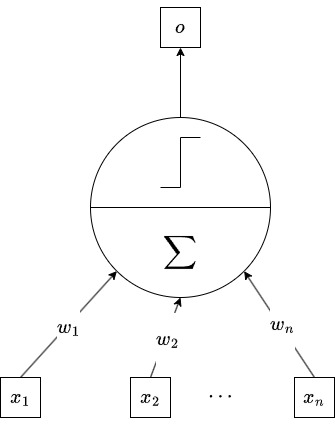
\includegraphics[width=0.5\linewidth]{img/img-perceptron}
			\caption{The perceptron}
			\label{fig:img-perceptron}
		\end{figure}
		
		
		A simple learning algorithm fits a perceptron to any linearly separable set.


		\bigskip
		\subsubsection{Multilayer perceptron}
		
		A multilayer perceptron is made up of fully connected layers. It contains an input layer, a number of hidden layers, and an output layer. This structure allows us to model more complex relationships when compared to the simpler perceptron. 
		
		The building blocks of a perceptron are the following:
		
		\begin{itemize}
			\item Each input feature is connected directly to an input neuron to forward the features into the network.
			\item One, or more than one, hidden layers, each having a designated number of nodes, follow. These layers transform the feature information at each level.
			\item Finally, an output layer consisting of one node (if the task is regression or binary classification) or more nodes (if the task is multi-class classification) gives us the result of the network.
		\end{itemize}
		\bigskip
		
		\begin{figure}[H]
			\centering
			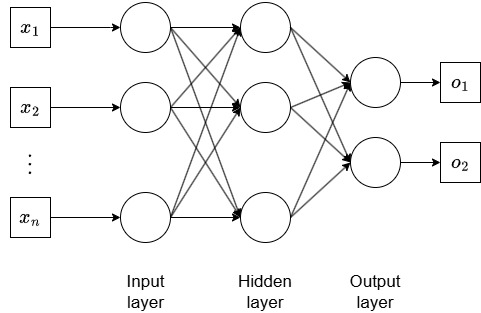
\includegraphics[width=0.7\linewidth]{img/img-multilayer-perceptron}
			\caption{A multilayer perceptron with a single hidden layer}
			\label{fig:img-multilayer-perceptron}
		\end{figure}
		\bigskip
		
		\begin{enumerate}
			\item Forward propagation involves feeding feature information to the input layer, passing it through all hidden layers, and finally to the output layer to generate a predicted output. A linear transformation followed by a non-linear activation generates the output for every node at each layer. Forward propagation is comprised of the following steps:
			
			\bigskip
			\begin{enumerate}
				\item For each neuron in layer $j$, the weighted sum of its inputs is calculated as:
				\begin{equation}
					z_j = \sum_{i=1}^{n_j} w_{ij}^{(j)} x_i^{(j-1)} + b_j
				\end{equation}

				Where:
				\begin{description}
					\item[$x_i^{(j-1)}$] Input from the $i^{th}$ neuron of the previous layer $j-1$.
					\item[$w_{ij}^{(j)}$] Weight connecting the $i^{th}$ neuron of layer $j-1$ to the current neuron in layer $j$.
					\item[$b_j$] Bias term for the neuron in layer $j$.
					\item[$z_j$] Result of the linear transformation at the current neuron in layer $j$.
					\item[$n_j$] Number of inputs (or neurons) in the previous layer $j-1$.
				\end{description}
				\bigskip
							
				\item The result of the weighted sum, $z_j$, is passed through a non-linear activation function:
				$$
				a_j = f(z_j)
				$$
				This introduces non-linearity to the model. A list of some common activation functions can be seen in the Table \ref{tab:activation_functions}.
				
				\begin{table}[H]
					\centering
					\begin{tabular}{|l|c|c|}
						\hline
						\textbf{Function} & \textbf{Equation} & \textbf{Diagram} \\ \hline\hline
						Sigmoid & 
						$\sigma(x) = \frac{1}{1+e^{-x}}$ & 
						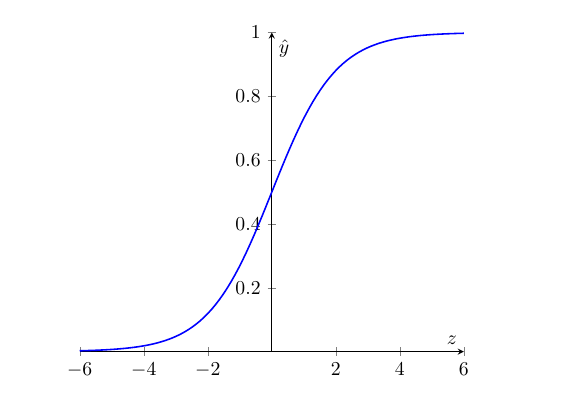
\includegraphics[width=0.3\linewidth]{img/img-neural-network-activation-functions-sigmoid} \\ \hline\\
						
						Tanh & 
						$tanh(x)$ & 
						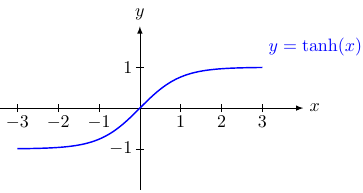
\includegraphics[width=0.3\linewidth]{img/img-neural-network-activation-functions-tanh} \\ \hline \\
						
						Leaky Relu & 
						$max(0.2x, x)$ & 
						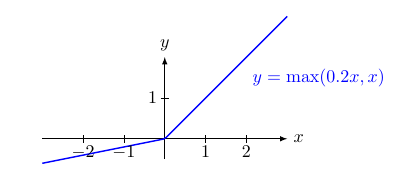
\includegraphics[width=0.3\linewidth]{img/img-neural-network-activation-functions-leaky-relu} \\ \hline \\
						
						Relu & 
						$max(0, x)$ & 
						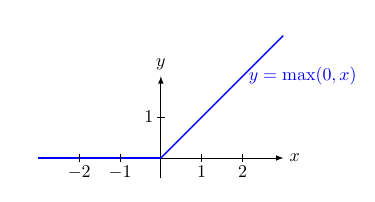
\includegraphics[width=0.3\linewidth]{img/img-neural-network-activation-functions-relu} \\ \hline 
					\end{tabular}
					\caption{Activation Functions}
					\label{tab:activation_functions}
				\end{table}
			\end{enumerate}
			\bigskip

			\item The predicted output is compared to the actual output using a loss function to compute the loss. A loss function measures the difference between the actual target values and the model's predicted results. For a single prediction:
			$$
			\text{Loss}(\hat{y}, y) = f(\hat{y}, y)
			$$
			Where:
			\begin{description}
				\item[$\hat{y}$] Predicted value.
				\item[$y$] Actual value.
				\item[$f$] Specific loss function formula.
			\end{description}
			\bigskip

			The cost function aggregates the loss over the entire dataset:
			$$
			\frac{1}{m} \sum_{i=1}^m \mathcal{L}(\hat{y}, y)
			$$
			
			\bigskip
			Two examples of cost functions are the following:
			\begin{itemize}
				\item Mean Squared Error (MSE):
				\begin{equation}
					\text{MSE} = \frac{\sum_{i=1}^n (\hat{y}^{(i)} - y^{(i)})^2}{n}
				\end{equation}

				
				\item Binary Cross-Entropy:
				Commonly used for binary classification problems:
				\begin{equation}
					L = -\frac{1}{N} \sum_{i=1}^N \left[ y_i \log(\hat{y}_i) + (1 - y_i) \log(1 - \hat{y}_i) \right]
				\end{equation}

				\bigskip
				Where:
				\begin{description}
					\item[$L$] The average loss (cost) across all $N$ samples in the dataset.
					\item[$y_i$] The true label for the $i^{th}$ sample, where $y_i \in \{0, 1\}$.
					\item[$\hat{y}_i$] Predicted probability for $y_i = 1$.
					\item[$1 - \hat{y}_i$] Predicted probability for $y_i = 0$.
					\item[$\log$] The natural logarithm.
				\end{description}
				\bigskip

			\end{itemize}
			\bigskip
			
			\item Backpropagation is the process by which the network's weights and biases are adjusted to minimize loss. The loss is propagated backwards from the output layer to the input layer. At each step, the gradient of the loss with respect to the parameters determines the adjustment. The following steps make up the backpropagation phase:
			
			\bigskip
			\begin{enumerate}
				\item The gradient of the loss with respect to each weight and bias in every node is calculated, starting from the output layer and moving backwards to the input layer.
				\item The gradient for any layer builds on the gradient of the subsequent (later) layers.
				\item The network's parameters for any node are adjusted in the direction opposite to the respective gradient using optimization algorithms like stochastic gradient descent (SGD) or variants such as the Adam optimizer.
			\end{enumerate}
		\end{enumerate}


		\bigskip
		\subsubsection{Stochastic gradient descent}
		
		Stochastic gradient descent is an optimization algorithm that optimizes the parameters $\Theta$ of the network, to minimize the loss
		
		$$
		\Theta = \arg \min_{\Theta}\frac{1}{N} \sum_{i=1}^{n}l(x_i, \Theta)
		$$

		Where:
		\[
		\begin{array}{ll}
			x_{1,2,\dots,N} & \text{The training set.} \\
			l(x_i, \Theta) & \text{The loss for a given data point } x_i. \\
			N & \text{The number of examples in the dataset.}
		\end{array}
		\]
		\bigskip
		
		As Wu noted\cite{wu2017introduction}, the loss, $z$ is a supervision signal that guides any modifications that should take place on the parameters. The stochastic gradient descent method of such modification is as follows:
		
		$$
		\theta^i\leftarrow \theta^i - \eta \frac{\partial z}{\partial \theta^i}
		$$
		where 
		$i$ represents the layer index
		$\eta$ is the learning rate
		$\frac{\partial z}{\partial \theta^i}$ is the gradient of the loss $z$ with respect to parameter $\theta^i$
		
		The parameters are updated iteratively,  as follows:
		
		$$
		\theta^i_{t+1} = \theta^i_{t} - \eta \frac{\partial z}{\partial \theta^i_{t}}
		$$
		
		There are a few considerations that are important to note about stochastic gradient descent.
		
		The learning rate affects the step size for each update, that is how much the parameters are adjusted in the direction of the gradient. A large learning rate might result in overshooting and even divergence, whereas a small learning rate leads to more stable convergence, albeit slower
		
		The parameters are updated for every sample or for a small batch of samples, unlike traditional gradient descent that computes that gradients for the entire dataset. This approach leads to faster updates but is also prone to more noise in the optimization process.
		
		
		
		\bigskip
		\subsubsection{Momentum}
		\label{section:momentum}
		
		Momentum is a technique used in training neural networks to accelerate optimization. This accelerated optimization is achieved by considering also the values of previous gradients for each parameter. Momentum can, in this way, mitigate oscillations in the optimization path and speed up learning.
		
		Momentum acts on the update rule of gradient descent by adding a portion of the update from the previous step to the current step. This approach allows the optimizer to maintain a directional memory, or velocity, effectively smoothing out updates and reducing oscillations.
		
		Momentum is commonly integrated with optimization algorithms like SGD and is a key component of advanced optimizers like Adam optimizer in Section \ref{section:adam}.
		
		The momentum update rule is given by:
		
		$$
		v^i_t = \beta v^i_{t-1} + (1 - \beta)\frac{\partial z}{\partial \theta^i_{t}}
		$$
		$$
		\theta^i_{t+1} = \theta^i_t - \eta v^i_t
		$$
		
		Where:
		\begin{description}
			\item[$v^i_t$] The velocity term at step $t$ for the parameters at index $i$.
			\item[$\beta$] The momentum coefficient (e.g., $0.9$), controlling how much of the previous velocity to retain.
			\item[$\frac{\partial z}{\partial \theta^i_{t}}$] The gradient of the loss function $z$ with respect to parameters $\theta^i$ at step $t$.
			\item[$\eta$] The learning rate.
			\item[$\theta^i_t$] The parameters at layer index $i$ at step $t$.
		\end{description}
		\bigskip

		
		
		A typical value is $\beta = 0.9$, which retains 90\% of the previous velocity. Smaller values result in less "memory" of past updates.  


		\bigskip
		\subsubsection{RMSProp}
		\label{section:RMSProp}
		
		Root Mean Square Propagation (RMSProp) is an adaptive learning rate optimization algorithm designed to improve the training of neural networks. Its main function is to address challenges such as inconsistent or large gradient magnitudes. RMSProp helps stabilize convergence during optimization due to its effectiveness in dealing with noisy gradients.
		
		RMSProp adjusts the learning rate for each parameter based on the average of recent squared gradients. In this way, the optimizer adapts to the scale of the gradients, preventing large updates that could destabilize training.  
		
		The algorithm is similar to [[neural-network-momentum]], but here it introduces a running average of squared gradients to normalize parameter updates.
		
		The RMSProp update rule is given by:
		
		\begin{equation}
			S^i_t = \beta S^i_{t-1} + (1 - \beta) \left( \frac{\partial z}{\partial \theta^i_{t}} \right)^2
		\end{equation}

		
		Where:
		\begin{description}
			\item[$S^i_t$] Exponentially weighted moving average of squared gradients at step $t$ for the parameters at layer index $i$.
			\item[$\beta$] Decay rate for the moving average (commonly set to $0.9$).
			\item[$\left( \frac{\partial z}{\partial \theta^i_{t}} \right)^2$] Gradient of the loss function $z$ with respect to parameters $\theta^i_t$ at step $t$ and layer index $i$.
		\end{description}
		\bigskip
		
		
		The parameters are updated using a learning rate scaled by the square root of $S^i_t$ (with a small value $\epsilon$ added for numerical stability):
		
		\begin{equation}
			\theta^i_{t+1} = \theta^i_t - \frac{\eta}{\sqrt{S_t + \epsilon}} 
			\left( \frac{\partial z}{\partial \theta^i_{t}} \right)
		\end{equation}
		
				
		Where:
		\begin{description}
			\item[$\eta$] Global learning rate, which is set to $0.001$ in most frameworks.
			\item[$\epsilon$] Small constant (e.g., $10^{-8}$) to prevent division by zero.
		\end{description}
		\bigskip

		
		RMSProp is a widely used optimizer that forms the foundation for more advanced methods such as adam optimizer that is discussed in detail in Section \ref{section:adam}. It is especially effective in training deep neural networks where gradient magnitudes can vary significantly.

	
		\bigskip
		\subsubsection{Adam optimizer}
		\label{section:adam}
		
		The Adam Optimizer (Adaptive Moment Estimation) is a widely used optimization algorithm for training deep learning models. It combines the benefits of momentum and rmsprop to provide an efficient, robust, and adaptable optimizer. Adam is particularly effective for problems with sparse gradients and non-stationary objectives.
		
		
		Adam optimizer had a number of hyper parameters:
		
		\begin{itemize}
			\item Learning Rate $\alpha$: \texttt{0.001}
			\item First Moment Decay Rate $\beta_1$: \texttt{0.9}
			\item Second Moment Decay Rate $\beta_2$: \texttt{0.999}
			\item Numerical Stability Term $\epsilon$: \texttt{1e-8}
		\end{itemize}
		\bigskip

		
		The Adam-optimizer update rule is given by the following steps:
		\bigskip
		\begin{enumerate}
			\item First, calculate the first moment estimate, or the Momentum that we discussed in Section \ref{section:momentum}, which is the exponentially weighted moving average of the gradients. This is done to smooth gradient updates over time by including past gradients and thus maintaining a directional memory:
			$$
			m^i_t = \beta_1 m^i_{t-1} + (1 - \beta_1)\frac{\partial z}{\partial \theta^i_{t}}
			$$
			
			\item Calculate the second moment estimate, which is the basic idea of RMSProp that we discussed in Section \ref{section:RMSProp}, to track the exponentially weighted variance of gradients:
			$$
			v^i_t = \beta_2 v^i_{t-1} + (1 - \beta_2) \left( \frac{\partial z}{\partial \theta^i_{t}} \right)^2
			$$
			
			\item Correct these results for initialization bias:
			$$
			\hat{m}^i_t = \frac{m^i_t}{1 - \beta_1^t}
			$$
			$$
			\hat{v}^i_t = \frac{v^i_t}{1 - \beta_2^t}
			$$
			
			\item Update the parameters using the corrected estimates:
			$$
			\theta^i_{t+1} = \theta^i_t - \frac{\alpha \hat{m}^i_t}{\sqrt{\hat{v}^i_t} + \epsilon}
			$$
		\end{enumerate}


		\bigskip
		\subsubsection{Batch normalization}
		
		Batch normalization is used to control the statistics of the activations in the neural networks. It is commonly used in neural network architectures, and it is usually found after layers that have multiplications, like linear or convolutional layers 
		
		Let us consider a hidden state neural net node
		
		We have basically a pre-activation value, that is the result of 
		
		$$
		z = \left(\sum_{i=1}^{n} x_i w_i \right)+ b
		$$
		
		That is fed into a non-linear element such as RELu or tanh.
		
		\begin{itemize}
			\item We do not want the pre-activation to be very small as the tanh activation will not effectively activate.
			\item We also do not want these values to be too large, as the tanh will become saturated.
			\item Furthermore, we want these values to be roughly Gaussian, that is, with a mean of 0 and a standard deviation of 1.
		\end{itemize}
		\bigskip
		
		Sergey Ioffe and Christian Szegedy propose batch-normalization \cite{ioffe2015batch} to take the hidden states and normalize them to be Gaussian.
		
		\begin{figure}
			\centering
			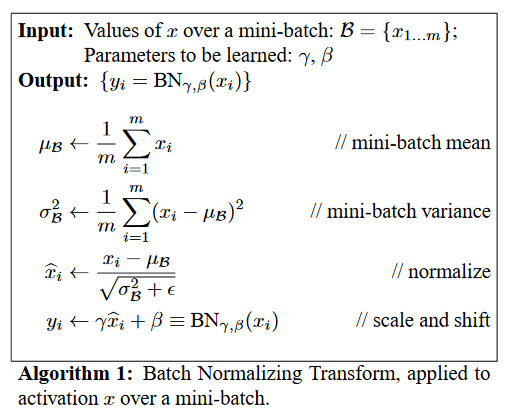
\includegraphics[width=0.7\linewidth]{img/img-ioffeBatchNormalizationAccelerating2015-1}
			\caption{Batch normalization algorithm, from \cite{ioffe2015batch}}
			\label{fig:img-ioffebatchnormalizationaccelerating2015-1}
		\end{figure}
		

		
		There are two ways whereby batch normalization can be implemented:
		
		\begin{itemize}
			\item Pre-activation normalization, where batch-normalization is carried out before the activation function is applied.
			\item Post-activation normalization, where batch-normalization is carried out after the activation function is applied.
		\end{itemize}
		\bigskip
		
		The original paper specified pre-activation normalization, however studies have shown that post-activation batch normalization will give superior results.



		\bigskip
		\subsubsection{Regularization}
		
		Regularization are techniques used to prevent overfitting in machine learning. This is achieved by adding a penalty term to the [[loss-function]], that discourage the model from assigning larger weights to features.
		
		L1 regularization or Lasso Regularization adds the sum of the absolute values of the weights to the [[loss-function]]:
		
		\begin{equation}
			\mathcal{L}_{L1} = \mathcal{L} + \lambda \sum_{i=1}^n |w_i|
		\end{equation}

		
		Where:
		\begin{description}
			\item[$\mathcal{L}$] The original loss function (e.g., cost-function-mean-square-error, cost-function-cross-entropy).
			\item[$\lambda$] The regularization strength, a hyperparameter.
			\item[$w_i$] The weight of the $i^{th}$ node.
		\end{description}
		\bigskip
		
		L1 regularization drives some weights to zero, thus encouraging sparsity in the network. Since L1 penalizes large weights, it promotes simpler networks with improved generalization.
		
		L2 or Ridge regularization adds the sum of the squared values of the weights to the [[loss-function]]:
		

		\begin{equation}
			\mathcal{L}_{L2} = \mathcal{L} + \lambda \sum_{i=1}^n w_i^2
		\end{equation}
		
		Where:
		\begin{description}
			\item[$\mathcal{L}$] The original loss function (e.g., cost-function-mean-square-error, cost-function-cross-entropy).
			\item[$\lambda$] The regularization strength, a hyperparameter.
			\item[$w_i$] The weight of the $i^{th}$ node.
		\end{description}
		\bigskip
		
		
		L2 penalizes large weights but does not drive them to zero but shrinks them closer to zero. It hence promotes smoother solutions and avoids sharp changes in parameter values.



	%% logistic regression
	%% -------------------

	\bigskip
	\subsection{Machine learning technique - Logistic regression}

		
		Logistic regression is a machine learning algorithm commonly used for binary classification tasks.
		
		Given a feature vector $X \in \mathbb{R}^{n_x}$, the goal of logistic regression is to predict the probability $\hat{y}$ that a binary output variable $y$ takes the value 1, given $X$, that is $\hat{y} = P(y=1|X)$, $0\le y\le1$. 
		For example, in the case of image classification, logistic regression can be used to predict the probability that an image contains a cat.
		
		\begin{figure}[H]
			\centering
				\begin{tikzpicture}
		\usetikzlibrary{calc}
		% Draw the ellipse
		\draw  (-0,0) circle (2);
		% Node at the center of the ellipse
		\node[circle, inner sep=0pt] (v2) at (-0,0) {};
		% Nodes for the lines
		\node (v1) at (-5, 2) {$x_1$};
		\node (v3) at (-5,0) {$x_2$};
		\node (v4) at (-5,-2) {$x_n$};
		\node (v7) at (4,0) {$\hat{y}$};
		% Draw lines stopping at the ellipse
		\draw[-] (v1) -- ($(v2)!0.37!(v1)$);
		\draw[-] (v3) -- ($(v2)!0.4!(v3)$);
		\draw[-] (v4) -- ($(v2)!0.37!(v4)$);
		\draw[-] (v7) -- ($(v2)!0.5!(v7)$);
		\node (v5) at (0,2) {};
		\node (v6) at (0,-2) {};
		\draw  (v5) edge (v6);
		\node [font=\tiny] at (-1,0) {$z=\textbf{W}^T\textbf{X}+b$};
		\node [font=\tiny] (v8) at (1,0) {$\hat{y}=\sigma(z)$};
		\node at (-3,1.5) {$w_1$};
		\node at (-3,0.25) {$w_2$};
		\node at (-3,-1.5) {$w_n$};
		\node at (-3,-0.5) {$\vdots$};
\end{tikzpicture}

			\caption{A logistic regression model}
			\label{fig:logisticregression}
		\end{figure}
		
		
		Logistic regression can be visualized as the model shown in Figure \ref{fig:logisticregression}. It consists of several main components:
		
		\begin{itemize}[]
			\item Inputs. The input vector to the model $\textbf{X} \in \mathbb{R}^{n_x}$.
			
			\item Parameters. A weight vector $\textbf{W} \in \mathbb{R}^{n_x}$ and a bias term $b \in \mathbb{R}$.  These will form the coefficients of a linear equation that gives the log odds ratio.
			
			\item Pre-activation result: The result is obtained by multiplying the transpose of the weights with the inputs and then adding the bias. 
			\begin{equation}
				z = \textbf{W}^{T}\textbf{X} + b = 
				\begin{bmatrix} 
					w_1 & w_2 & \dots & w_n
				\end{bmatrix}
				\begin{bmatrix} 
					x_1 \\ 
					x_2 \\ 
					\vdots \\ 
					x_n
				\end{bmatrix} + b
			\end{equation}

			
			
			\item Sigmoid function. A function as shown in Figure \ref{fig:sigmoid}, $\sigma(z) = \frac{1}{1 + e^{-z}}$, which maps any real number $z$ to the range $(0,1)$. This function is used to ensure that the predicted probability $\hat{y}$ is always between 0 and 1.
			
			\begin{figure}[H]
				\centering
				 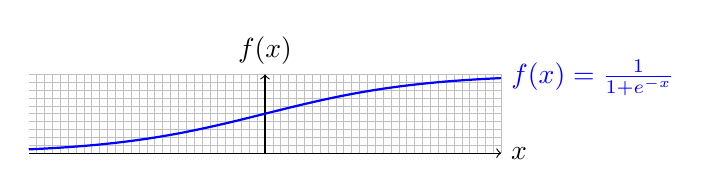
\begin{tikzpicture}[domain=-3:3] [H]% Reduced domain for a narrower plot
	% Grid and axes
	\draw[very thin,color=lightgray, step=0.1] (-3,-0) grid (3,1);
	\draw[->] (-3,0) -- (3,0) node[right] {$x$};
	\draw[->] (0,-0) -- (0,1) node[above] {$f(x)$};
	
	% Sigmoid function
	\draw[color=blue, thick, samples=100] 
	plot (\x, {1/(1 + exp(-\x))}) 
	node[right] {$f(x) = \frac{1}{1 + e^{-x}}$};
\end{tikzpicture}

				\caption{Sigmoid activation function}
				\label{fig:sigmoid}
			\end{figure}
			
			\item Output. The predicted probability $\hat{y}$ is computed as $\hat{y} = \sigma(z) = \sigma(\textbf{W}^{T}\textbf{X} + b)$.
		\end{itemize}
		\bigskip
		
		
		A term that is often encountered in this scenario is the log-odds ratio or logit. Logistic regression models the probability $P(y = 1 \mid X)$, of the binary dependent variable $Y$ given the predictor variables $\textbf{X} = \{x_1, x_2, \dots, x_n\}$. The goal is to find a relationship between $P(y=1)$, and the predictors $\textbf{X}$.
		
		The probability is modelled using the sigmoid function:
		$$P(y = 1 \mid X) = \frac{1}{1 + e^{-\eta}}$$
		
		Where:
		$\eta = b + w_1 x_1 + w_2 x_2 + \dots + w_n x_n$  is the linear regression function
		
		The odds of $y=1$ are defined as the ratio of the probability of success to the probability of failure:
		
		$$\text{Odds} = \frac{P(y = 1)}{1 - P(y = 1)}$$
		
		Taking the natural logarithm of the odds gives the 
		[log-odds-ratio]] or logit:
		
		$$\text{Log-Odds} = \ln\left(\frac{P(y = 1)}{1 - P(y = 1)}\right)$$
		
		From the sigmoid function, we can derive the relationship between the probability and the log-odds-ratio:
		
		$$P(y = 1) = \frac{1}{1 + e^{-\eta}}$$
		$$1 - P(y = 1) = 1 - \frac{1}{1 + e^{-\eta}} = \frac{e^{-\eta}}{1 + e^{-\eta}}$$
		
		The odds, therefore, are
		$$\text{Odds} = \frac{P(y = 1)}{1 - P(y = 1)} = \frac{\frac{1}{1 + e^{-\eta}}}{\frac{e^{-\eta}}{1 + e^{-\eta}}} = e^{\eta}$$
		
		
		Taking the natural logarithm of both sides gives the log-odds:
		
		$$ln\left(\frac{P(y = 1)}{1 - P(y = 1)}\right) = \eta$$
		
		Substituting $\eta = b + w_1 x_1 + w_2 x_2 + \dots + w_n x_n$
		
		\begin{equation}
			\ln\left(\frac{P(y = 1)}{1 - P(y = 1)}\right) = \eta = b + w_1 x_1 + w_2 x_2 + \dots + w_n x_n
		\end{equation}
		
		\bigskip
		
		We conclude this overview of logistic regression by looking at how they work and learn.	The weight vector $\textbf{W}$ and the bias term $b$ are learned from a labelled training set by minimizing a suitable loss function using techniques such as gradient descent or its variants. Once trained, the logistic regression model can be used to predict the probability of the binary output variable for new input examples.
		
		
		The feedforward process for logistic regression can be described as follows:
		
		\begin{enumerate}[]
			\item Compute $z$ as the dot product of the weight vector $\textbf{W}$ and the input features, plus the bias term $b$, transforming the input features info a single scalar $z$ that represents the log-odds of the output being $y=1$: 
			\begin{equation}
				z= \textbf{W}^{T}\textbf{X} + b
			\end{equation}
			
			\item Pass $z$ through the sigmoid function to map the log-odds $z$ to a probability $\hat{y} = P(y = 1 \mid X)$, ensuring the output is between 0 and 1: 
			\begin{equation}
				\hat{y} = \sigma(z) = \frac{1}{1 + e^{-z}}
			\end{equation}
			
			\item During training, we define the loss function $\mathcal{L}$ as the negative log-likelihood of the predicted output given the true label: 
			\begin{equation}
				\mathcal{L} = -\left(y\ln(\hat{y}) + (1-y)\ln(1-\hat{y})\right)
			\end{equation}
		\end{enumerate}
		
		For a trained system, we compare $\hat{y}$ to a threshold to convert the probabilistic output into the final binary classification.
		
		\bigskip
		
		We now look at \textbf{feedback process} for logistic regression. To optimize the weight vector $\textbf{W}$, we compute the derivatives of the loss function with respect to each weight and the bias term and use these derivatives to update the weights in the opposite direction of the gradient. This is known as gradient descent.
		
		To compute the derivatives, we use the chain rule:
		
		$$
		\frac{\partial\mathcal{L}}{\partial w_i} =
		\frac{\partial\mathcal{L}}{\partial \hat{y}} \cdot
		\frac{\partial \hat{y}}{\partial z} \cdot
		\frac{\partial z}{\partial w_i}
		$$ and
		$$
		\frac{\partial\mathcal{L}}{\partial b} =
		\frac{\partial\mathcal{L}}{\partial \hat{y}} \cdot
		\frac{\partial \hat{y}}{\partial z} \cdot
		\frac{\partial z}{\partial b}
		$$
		
		We can then use these derivatives to update the weights as follows:
		
		
		\begin{equation}
			w_i \leftarrow w_i - \alpha \frac{\partial \mathcal{L}}{\partial w_i}
		\end{equation}
		
		and
		
		\begin{equation}
			b \leftarrow b - \alpha \frac{\partial \mathcal{L}}{\partial b}
		\end{equation}
		
		
		Where $\alpha$ is the learning rate, which controls the step size of the updates. By iteratively performing these updates on a training set, we can find the optimal weight vector $\textbf{W}$ that minimizes the loss function on the training set.
		
		\bigskip
		
		To calculate the derivatives, let us begin by computing the derivative of the loss function with respect to the predicted output $\hat{y}$:
		
		
		$$
		\frac{\partial \mathcal{L}}{\partial\hat{y}} = 
		\frac{\partial}{\partial\hat{y}} 
		\left(  
		-\left(y\ln(\hat{y}) + (1-y)\ln(1-\hat{y})\right)
		\right) 
		$$
		since 
		$$\frac{d \space (ln (x))}{dx}  = \frac{1}{x}$$we get:
		$$\frac{\partial \mathcal{L}}{\partial \hat{y}} = - \left( \frac{y}{\hat{y}} - \frac{1-y}{1-\hat{y}} \right) $$
		
		The derivative of the predicted output $\hat{y}$ with respect to $z$ is solved using the quotient rule, that is 
		$$
		\frac{d}{dx} \left( \frac{f(x)}{g(x)} \right) = \frac{f'(x)g(x) - g'(x)f(x)}{g^2(x)}
		$$
		
		So, if we let
		
		\begin{table}[!ht]
			\centering
			\begin{tabular}{|l|l|l|}
				\hline
				$f(z) = 1$ & $f'(z) = 0$ \\ \hline
				$g(z)=1 +e^{-z}$ & $g'(z)= -e^{-z}$ \\ \hline
			\end{tabular}
		\end{table}
		
		
		\begin{align*}
			\frac{\partial\hat{y}}{\partial z} 
			& = \frac{\partial}{\partial z} \left( \frac{1}{1 + e^{-z}} \right) \\
			& = \frac{e^{-z}}{(1 + e^{-z})^2} \\
			& = \frac{1}{(1 + e^{-z})} \space \frac{e^{-z}}{(1 + e^{-z})} \\
			& = \frac{1}{(1 + e^{-z})} \space \frac{1 + e^{-z} -1}{1 + e^{-z}} \\
			& = \frac{1}{(1 + e^{-z})} \space \left( \frac{1 + e^{-z}}{1 + e^{-z}} - \frac{1}{1 + e^{-z}} \right)\\
			& = \hat{y}(1-\hat{y})\\
		\end{align*}
		
		
		
		The derivative of $z$ with respect to $w_i$:
		
		\begin{equation}
			\begin{split}
				\frac{\partial z}{\partial w_i} 
				&=	\frac{\partial}{\partial w_i} \textbf{W}^T \textbf{X} + b\\
				&= 	\frac{\partial}{\partial w_i} (w_1 x_1 + \dots + w_ix_i+\dots+w_nx_n + b)\\
				&= x_i\\
			\end{split}
		\end{equation}
		
		Similarly,
		
		
		\begin{equation}
			\begin{split}
				\frac{\partial z}{\partial b} 
				&= \frac{\partial}{\partial b} \textbf{W}^T \textbf{X} + b\\
				&= 	\frac{\partial}{\partial b} (w_1 x_1 + \dots + w_ix_i+\dots+w_nx_n + b)\\
				&= 1\\
			\end{split}	
		\end{equation}	
		
		Therefore
		
		
		\begin{align*}
			\frac{\partial\mathcal{L}}{\partial w_i} 
			&= \frac{\partial\mathcal{L}}{\partial \hat{y}} \cdot
			\frac{\partial \hat{y}}{\partial z} \cdot
			\frac{\partial z}{\partial w_i} \\
			& = 
			-\left(
			\frac{y}{\hat{y}} - \frac{1-y}{1-\hat{y}}
			\right) \cdot
			\hat{y}(1-\hat{y})
			\cdot
			x_i\\
			&= 
			-\left(
			\frac{-y(1-\hat{y}) + (1-y)\hat{y}}{\hat{y}(1-\hat{y})}
			\right) \cdot
			\hat{y}(1-\hat{y})
			\cdot
			x_i\\
			&= \left[ (1-y)\hat{y} -y(1-\hat{y})  \right]x_i\\
			&= \left[ \hat{y} -y\hat{y} -y +y\hat{y}\right]x_i\\
		\end{align*}
		\begin{equation}
			\frac{\partial\mathcal{L}}{\partial w_i} = (\hat{y} - y) x_i
		\end{equation}
		
		and similarly
		
		\begin{equation}
			\frac{\partial\mathcal{L}}{\partial b} =
			\left(
			\hat{y} - y
			\right)
		\end{equation}
		

	%% knn
	%% ---
	
	\bigskip
	\subsection{Machine learning technique - K-nearest neighbours algorithm}
	
	K-nearest neighbours is simple yet robust for datasets with well-structured local relationships. It is particularly effective for non-linear decision boundaries and finds applications in anomaly detection, pattern recognition, and recommendation systems.
	
	The k-nearest neighbours algorithm is non-parametric, that is, it does not make assumptions about the underlying distribution or functional form of the data; instance-based, that is, it does not explicitly learn a model during a training phase, but it relies on the raw training data to make predictions at query time, unlike parametric models, which "learn" a set of fixed parameters (e.g., coefficients in linear regression) during training,   learning method used for classification and regression tasks. It predicts the output of a query point based on the labels or values of its $k$-nearest neighbours in feature space.
	
	KNN does not assume a specific functional form for the data. Instead, it relies on the local structure of the dataset. For a given query point $x$, the algorithm uses a distance metric to identify its $k$-nearest neighbours and infers the prediction by aggregating their outcomes. Typical distance metrics include:
	\begin{enumerate}
		\item Euclidean Distance
		$$
		d(x, x') = \sqrt{\sum_{i=1}^{n} (x_i - x'_i)^2}
		$$
		
		\item Manhattan Distance
		$$
		d(x, x') = \sum_{i=1}^{n} |x_i - x'_i|
		$$
		
		\item Minkowski Distance. Note that for $p = 2$, this reduces to the Euclidean distance; for $p = 1$, it becomes the Manhattan distance.
			$$
			d(x, x') = \left( \sum_{i=1}^{n} |x_i - x'_i|^p \right)^{1/p}
			$$
		\end{enumerate}
		
		
		In classification tasks, the predicted class  $\hat{y}$ for a query point $x$ is determined by majority voting among its  $k$-nearest neighbours. If we let $N_k(x)$ represent the set of the $k$-nearest neighbours,he predicted class is given by:
		
		$$
		\hat{y} = \text{argmax}_c \sum_{x' \in N_k(x)} \mathbb{I}(y(x') = c)
		$$
		
		Where:
		$$
		\begin{array}{ll}
			\text{argmax}_c & \parbox[t]{0.4\textwidth}{Identifies the class $c$ with the highest count among the neighbours.} \\
			\mathbb{I}(\cdot) & \parbox[t]{0.4\textwidth}{The indicator function, which equals  1 if  $y(x') = c$,  and 0 otherwise.}
		\end{array}
		$$

		
		The parameter $k$ determines the number of neighbours considered.
		
		\begin{itemize}
			\item A small $k$ (e.g., $k = 1$) makes the model sensitive to noise, as predictions rely heavily on individual points.
			\item A large $k$ smooths the decision boundary but may lead to underfitting.
		\end{itemize}
				
		Finding the optimal value for $k$ is one of the main challenges in the k-nearest neighbour. Cross-validation is typically employed to find a value using the following procedure:
		
		\bigskip
		\begin{enumerate}
			\item Iterate Over Candidate Values of $k$
			\begin{itemize}
				\item Choose a range of potential $k$ values, for example, $k = 1, 2, \dots, 20$.
			\end{itemize}
			
			\item Evaluate Performance for Each $k$
			\begin{itemize}
				\item For each $k$, use $K$-fold cross-validation:
				\begin{itemize}
					\item Train the KNN model using $K-1$ folds.
					\item Validate it on the remaining fold.
					\item Compute the average performance metric across all $K$ folds.
				\end{itemize}
			\end{itemize}
			
			\item Select $k$ with the Best Performance
			\begin{itemize}
				\item After evaluating all $k$ values, choose the $k$ that maximizes the performance metric (e.g., accuracy) or minimizes the error.
			\end{itemize}
		\end{enumerate}
		\bigskip
		
		The $k$-nearest neighbour algorithm is, therefore, as follows;
		
		\bigskip
		\subsubsection{Input}
		\begin{itemize}
			\item Dataset: $D = \{(x_1, y_1), (x_2, y_2), \dots, (x_N, y_N)\}$, where $x_i$ is the feature vector, and $y_i$ is the corresponding label or value.
			\item Query point: $x_{query}$, the data point for which the prediction is required.
			\item Number of neighbours: $k$, the number of nearest neighbours to consider.
			\item Distance metric: $d(x, x')$ (e.g., Euclidean distance).
		\end{itemize}
		
		\subsubsection{Steps:}
			\begin{enumerate}
			
			\item Calculate Distance. For the query point $x_{query}$, compute the distance to every point $x_i$ in the dataset $D$ using the chosen distance metric. For Euclidean distance:
			$$
			d(x_{query}, x_i) = \sqrt{\sum_{j=1}^{n} (x_{query_j} - x_{i_j})^2},
			$$
			$$
			\quad \forall i \in \{1, 2, \dots, N\}.
			$$
			
			\item Sort Neighbours. Rank all data points $x_i$ in $D$ by their distance to $x_{query}$ in ascending order. Let this sorted set be $D_{sorted}$.
			
			\item Select $k$-Nearest Neighbours. Extract the top $k$ data points from $D_{sorted}$. Denote this set as $N_k(x_{query})$.
			
			\item Aggregate Neighbours' Outputs.
			\begin{itemize}
				\item For \textbf{classification}: Perform majority voting among the labels $y_i$ of the $k$-nearest neighbours:
				$$
				\hat{y} = \text{argmax}_c \sum_{x_i \in N_k(x_{query})} \mathbb{I}(y_i = c),
				$$
				where $\mathbb{I}(y_i = c)$ is an indicator function that equals $1$ if $y_i = c$, and $0$ otherwise.
				
				
			\end{itemize}
			
			\item \textbf{Output Prediction:}
			Return $\hat{y}$ as the predicted label (for classification) or value (for regression) for $x_{query}$.
			
		\end{enumerate}
		
		\subsubsection{Output:}
		The predicted label or value $\hat{y}$ for the query point $x_{query}$.
		
		
		
		
		
		
		
		

		
		





	% rescaling and optimization
	% --------------------------

	\subsection{Feature scaling}

		Feature scaling is an important data transformation process. It is a very important aspect of many machine learning algorithms including logistic regression, support vector machines and neural networks, as, the performance of such algorithms is adversely impacted when the numerical features have different scales. The two methods to transform features on the same scale are normalization and rescaling.
		
		During normalization or rescaling, values are scaled and shifted so that they are mapped onto the $[0,\space 1]$ interval. This is achieved by applying the following transformation;
		$$
		x_{normalized} = \frac{x - x_{min}}{x_{max}-x_{min}}
		$$
		Normalization is also sometimes referred to as min-max scaling.
		
		Standardization is particularly suited for algorithms that assume Gaussian distributions, like linear regression and logistic regression. It is achieved by first subtracting values from the mean so that the mean of the normalized values is zero, and then dividing by the standard deviation so that the variance of the normalized distribution is one. Thus;
		$$
		x_{standardized} = \frac{x - \mu}{\sigma}
		$$
		Unlike normalization, the range of standardization is not fixed, and this can sometimes be an issue if a value in the $[0,\space 1]$ interval is expected.  Standardization is however more resilient to the effect of outliers.
		
		Tree based machine learning models, like decision trees and random forests do not normally require feature scaling.


	% cross validation
	% ----------------
	
	\subsection{Cross-validation}
	
		Cross-validation is a technique that can be applied to any ML algorithm that is aimed to reduce overfitting by estimating how well each hypothesis generalizes to unseen data. In practice, a portion of the data is reserved for this purpose.
		
		The $K$-fold cross validation technique splits the dataset into $k$ folds, training that model on $k-1$ folds and testing on the remaining one. The test fold is rotated and the process is repeated so that each fold will act as the test set once. Metrics like mean square error are averaged across folds, ensuring a robust estimate.
		
		Therefore, if for example, we split the data into 10 folds, so that each fold will have $n/10$ records, we train the model on 9 folds and test on the remaining one. We then rotate the test fold and repeat this process 10 times. The final performance metric is computed as the mean of the metrics across the 10 folds.
		
		In stratified $K$-fold cross validation, the folds have the same proportion of the classes as in the original dataset.
		
		Other types of cross validation include Leave one out cross-validation, where each data point is used as a test set once.
	
	
	% dimentionality reduction and feature selection
	% ----------------------------------------------
	
	
	% quantitative measurements
	% -------------------------
	
	\subsection{Measurement}
	
		Quantitative measurements numerically represent attributes and are fundamental for evaluating machine learning models by providing an objective means to assess the model's performance. We can analyse the model's effectiveness by comparing model predictions to actual outcomes. Appropriate selection and reporting of measurement methods, including their reliability, validity, and potential biases, are essential to ensure accurate interpretation and meaningful results. This section will look at the measurements used in this study.
		
		The function used in machine learning and statistical modelling to quantify the difference between the predicted outputs of a model and the actual target values is called the loss function. It serves as a measure of the model's performance, guiding the optimisation process to improve predictions.
		
		For a single prediction:
		
		$$\text{Loss}(\hat{y}, y) = f(\hat{y}, y)$$
		Where:
		
		
		\begin{compactitem}
			\item [$\hat{y}$]: Predicted value.
			\item [$y$]: Actual value.
			\item [$f$]: Specific loss function formula
		\end{compactitem}
		
		\bigskip
		
		The aggregation of the loss function across the entire dataset is called the cost function so that;
		
		$$
		\text{Cost}(\hat{y}, y) = \frac{1}{N}\sum_{i=1}^{N} \mathcal{L}(\widehat{y}_i, y_i)
		$$
		
		In the problem we are considering, we will try to predict whether a person will recidivate given information about his or her previous criminal history is a binary classifier problem. A binary classifier is a function that can be applied to features $X$ such as $(x_1, x_2, x_3, \dots, x_n)$ and maps them to an output $Y$, where $Y \in \{0, 1\}$. It is a supervised learning technique; therefore, a test set is extracted from the available data to validate the model before being deployed in production.
		
		$$ f(x_1, x_2, x_3, \dots, x_n) = Y \in \{0, 1\}  $$
		
		The function will return a value between 0 and 1; therefore, a threshold value is operated to classify the result as true or false. The model will subsequently classify predictions as true or false according to the threshold value.
		
		
		For the classification problem that we have in hand, we will  primarily use the log-likelihood  cost function defined as:
		
		$$\mathcal{L}_{\text{log-likelihood}} = - \sum_{i=1}^N \left[ y_i \ln(\hat{y}_i) + (1 - y_i) \ln(1 - \hat{y}_i) \right]$$
		
		Negative log-likelihood focuses on the distance between the labels $y_i$ and the predicted probabilities $\hat{y}_i$. If we consider a sample where:
		
		\begin{itemize}
			\item $y_i$ is one and $\hat{y}_i$ is close to 1: $y_i \ln(\hat{y}_i)$ is close to zero, while $(1 - y_i) \ln(1 - \hat{y}_i)$ is zero, so that the resultant loss is close to zero.
			\item $y_i$ is 1 and $\hat{y}_i$ is far from 1: $y_i \ln(\hat{y}_i)$ is large, while $(1 - y_i) \ln(1 - \hat{y}_i)$ is zero so that the resultant loss is large.
			\item $y_i$ is zero and $\hat{y}_i$ is close to 0: $y_i \ln(\hat{y}_i)$ is zero, while $(1 - y_i) \ln(1 - \hat{y}_i)$ is also close to zero so that the resultant loss is close to zero.
			\item $y_i$ is zero and $\hat{y}_i$ is far from 0: $y_i \ln(\hat{y}_i)$ is zero, while $(1 - y_i) \ln(1 - \hat{y}_i)$ is large so that the resultant loss is large.
		\end{itemize}
		\bigskip
		
		In this scenario,  we can obtain four kinds of results:
		
		\begin{table}[!ht]
			\centering
			\begin{tabular}{|l|l|l|p{2cm}|}
				\hline
				Prediction & Classif & Outcome & Description \\ \hline\hline
				1 & 1 & True Positive (TP) & The model correctly predicted the positive class. \\ \hline
				1 & 0 & False Positive (FP) & The model incorrectly predicted the positive class (a false alarm). \\ \hline
				0 & 1 & False Negative (FN) & The model incorrectly predicted the negative class (a miss). \\ \hline
				0 & 0 & True Negative (TN) & The model correctly predicted the negative class. \\ \hline
			\end{tabular}
		\end{table}
		
		The number of samples that are TP, TN, FP or FN can be organised in what is known as a confusion matrix, that is shown in Figure \ref{fig:confusionmatrix}. This tool makes it easy to perform calculations that determine the validity of the model at hand.
		
		\begin{figure}[H]
			\centering
			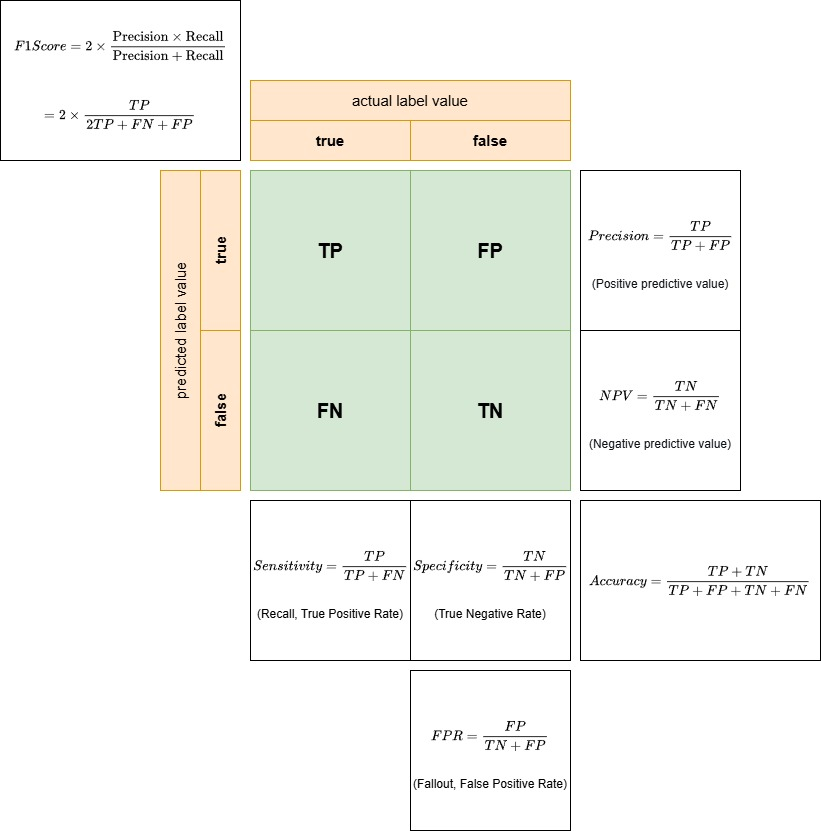
\includegraphics[width=0.9\linewidth]{img/confusion_matrix}
			\caption{Confusion matrix and associated equations}
			\label{fig:confusionmatrix}
		\end{figure}
		
		
		There are several key performance metrics derived from the confusion matrix, each offering a different perspective on evaluating the effectiveness of a binary classification model.
		
		\bigskip
		
		The \textbf{accuracy} of a model is a straightforward measure that evaluates the proportion of correct predictions (both True Positives and True Negatives) out of the total number of predictions. It can be mathematically defined as:
		
		
		$$Accuracy=\frac{TP+TN}{TP+FP+TN+FN}$$
		
		for a dataset,
		$$
		Accuracy = \frac{1}{N} \sum_{i=1}^{N} 1(\hat{y}_i = y_i)
		$$
		
		
		\textbf{Precision} answers the question: "Out of all the observations predicted to be positive, how many were positive?" In other words, it measures the model's ability to avoid false positives.
		
		$$Precision=\frac{TP}{TP+FP}$$
		
		
		\textbf{Recall} or \textbf{sensitivity} measures the model's ability to correctly identify positive cases. It answers the question: "Out of all the actual positive instances, how many did the model correctly identify as positive?"
		
		
		$$Recall=\frac{TP}{TP + FN}$$
		
		\textbf{Specificity} measures the model's ability to identify negative cases correctly. It answers the question: "Out of all the actual negative instances, how many did the model correctly identify as negative?"
		
		The formula for specificity is:
		
		$$Specificity= \frac{TN}{TN + FP}$$
		
		The F1-score is the harmonic mean of [precision](model-performance-precision) and [recall](model-performance-recall). It provides a single metric that balances precision and recall, which is useful when there is an uneven class distribution or when false positives and false negatives are important.
		
		The formula for the F1 score is:
		
		\begin{align*}
			F1 
			&= 2 \times \frac{\text{Precision} \times \text{Recall}}{\text{Precision} + \text{Recall}}\\
			&= 2\times \frac{TP}{2TP+FN+FP}\\
		\end{align*}	
		
		\bigskip
		
		As can be seen in Figure \ref{fig:img-receiver-operator-characteristic-curve}, the ROC curve is plotted by varying the decision threshold of the classifier and plotting the corresponding values of FPR (on the x-axis) and sensitivity or TPR (on the y-axis). Each point on the ROC curve represents a (FPR, TPR) pair for a particular threshold value.
		
		\begin{figure}[H]
			\centering
			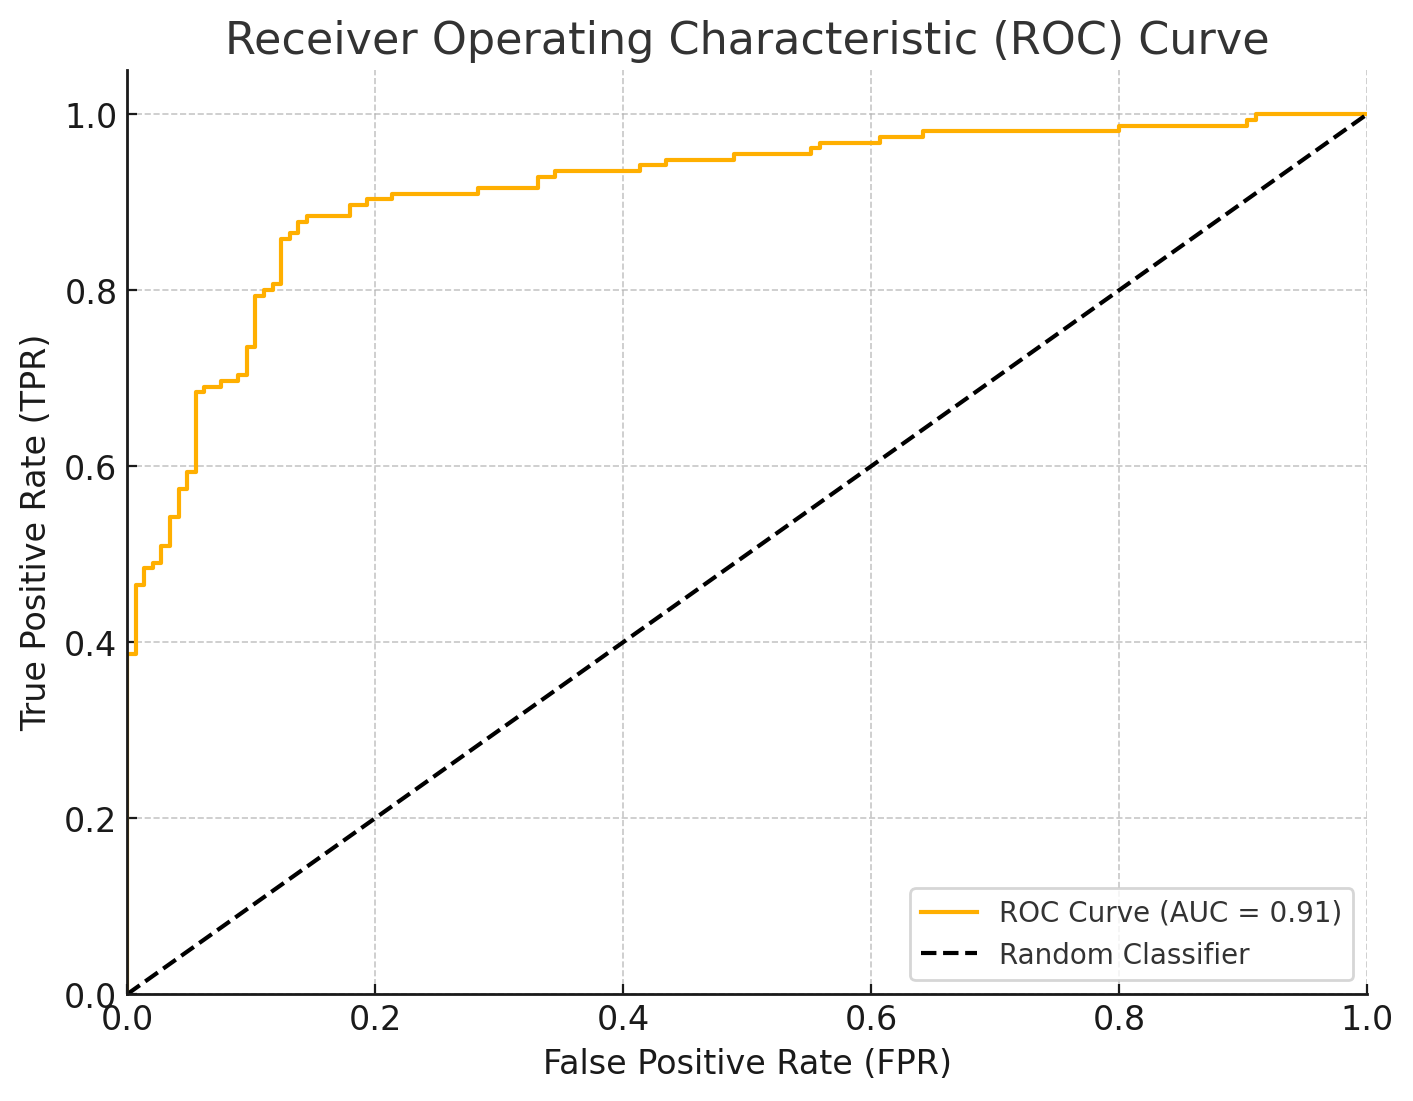
\includegraphics[width=0.7\linewidth]{img/img-receiver-operator-characteristic-curve}
			\caption{ROC curve}
			\label{fig:img-receiver-operator-characteristic-curve}
		\end{figure}
	
		The Area Under the ROC Curve (AUC) is a key indicator of model performance. The value of the AUC ranges from 0 to 1:
		
		
		\begin{itemize}
			\item A perfect classifier has an AUC of 1, indicating it achieves a TPR of 1 while keeping the FPR at 0.
			\item A model with an AUC of 0.5 performs no better than random guessing.
			\item Higher AUC values indicate better overall performance.
		\end{itemize}
		\bigskip
		
		The goal of a classifier is to maximise the TPR (correctly predicting positive instances) while minimising the FPR (incorrectly classifying negative instances as positive). Ideally, the ROC curve should approach the top-left corner of the plot, indicating a high TPR with a low FPR.
		
		In summary, the ROC curve helps to visualise and compare the trade-offs between true positives and false positives across different thresholds, and the AUC provides a single number summarising the model's ability to discriminate between positive and negative classes.
	
	

	
	%

\section{Data preparation}

%TODO add reference
The COMPAS dataset used in this study is publicly available through ProPublica's GitHub repository. This repository contains the dataset and other assets used by ProPublica to investigate the biases present in the COMPAS risk assessment tool.

The file chosen for this analysis is \textbf{\texttt{compas-scores-two-years.csv}}, as it provides the cleanest and most relevant data for general recidivism prediction. This CSV file contains the key data required for our study, including several attributes related to demographics, criminal history, COMPAS risk scores, and the two-year recidivism outcomes that are important for exploring the predictive capabilities and the ethical implications of machine learning models in the context of recidivism prediction. 

The dataset includes important information about individuals. Following an initial analysis, a list of the key fields in the dataset is below.

\begin{itemize}
	
	\item Personal Information, includes attributes such as \textbf{\texttt{age}}, \textbf{\texttt{race}}, \textbf{\texttt{age\_category}}, etc.
	
	\item Case and Event-Related Details are the fields prefixed with \textbf{\texttt{c\_}} that provide a timeline and details of a person's interactions with the criminal justice system.
	
	\item Violence Risk Assessment are the fields prefixed with \textbf{\texttt{v\_}} and are associated with the violence risk assessment in COMPAS. This dimension predicts violent recidivism risk.
	
	\item Case-Level Details for Violent Recidivism are the fields prefixed with \textbf{\texttt{vr\_}}. These fields provide additional details specific to violent recidivism events.
	
	\item Juvenile Criminal Record are the fields prefixed with \textbf{\texttt{juv\_}}. These fields capture information about an individual's juvenile criminal record, which is a key predictor of future adult criminal behaviour.
	
	\item Previous Charges and Severity can be deduced from fields such as \textbf{\texttt{priors\_count}} and \textbf{\texttt{juv\_}} fields.
	
	\item Additional fields, including \textbf{\texttt{r\_charge\_}}, \textbf{\texttt{r\_offense\_}}, \textbf{\texttt{vr\_}} fields, \textbf{\texttt{c\_charge\_degree}}, and \textbf{\texttt{c\_charge\_desc}}, provide a broader perspective on criminal history and severity.
	
	
	\item Two-Year Recidivism, or the \textbf{\texttt{two\_year\_recid}} field in the COMPAS dataset, indicates whether an individual reoffended (recidivated) within two years of their initial assessment or release. This field is critical for evaluating the predictive accuracy of the COMPAS risk assessment tool.
	
	\item Decile Score is a standardized risk score in the COMPAS dataset. It categorizes an individual's likelihood of recidivism into ten equal groups (deciles) where 1 is the lowest risk, and 10 is the highest risk. Each decile represents approximately 10\% of the sample when applied to a norm group.
	
\end{itemize}

%Suppose that we observe the following data:

%\begin{table}[!ht]
%	\centering
%	\begin{tabular}{|l|l|}
%		\hline
%		Field & Value \\ \hline
%		\textbf{\texttt{priors\_count}} & 5 \\ \hline
%		\textbf{\texttt{juv\_felony\_count}} & 2 \\ \hline
%		\textbf{\texttt{juv\_misdemeanor\_count}} & 3 \\ \hline
%		\textbf{\texttt{r\_charge\_degree}} & Felony \\ \hline
%	\end{tabular}
%\end{table}

%We can interpret this as an individual who has five total prior charges, including:

%\begin{itemize}
%	\item 2 juvenile felonies
%	\item 3 juvenile misdemeanours
%	\item The severity of previous charges includes felonies (\textbf{\texttt{r\_charge\_degree}}).
%\end{itemize}


\subsection{Preparing the data for further analysis and training}

Before we can perform any analysis or apply machine learning techniques, it is important to pre-process and prepare the dataset so that we can handle missing values, encode categorical features, and split the data into training, testing, and validation sets. This step will produce a clean dataset for building accurate and unbiased models. The following steps outline the procedures to prepare the dataset for further analysis and training.


\subsection{Initial look at data and missing values handling}

The dataset has 7214 instances over 53 columns. The COMPAS system risk factor is the field  \textbf{\texttt{decile\_score}}, but the dataset also contains information about whether or not the person recidivised through the label \textbf{\texttt{two\_year\_recid}}. 

The first step in this data analysis step was  removing the features irrelevant to this exercise or with over 50\% missing records. We removed all the COMPAS-administrative labels and additional recidivism information apart from \textbf{\texttt{two\_year\_recid}}, narrowing the dataset to 17 fields.

The difference between \textbf{\texttt{c\_jail\_in}} and \textbf{\texttt{c\_jail\_out}} was calculated into a new field, \textbf{\texttt{days\_in\_jail}} and the difference between \textbf{\texttt{in\_custody}} and \textbf{\texttt{out\_custody}}, in a new field, \textbf{\texttt{days\_in\_custody}}. We subsequently removed the features containing date information from the dataset, together with \textbf{\texttt{days\_in\_custody}}, as it contained no information. At this stage, the dataset contains thirteen features: eight numerical, four categorical, and one descriptive. It also contains two labels, decile\_score, which we will treat as the leading label in this exercise and \textbf{\texttt{two\_year\_recid}}, which we are keeping to compare the prediction power of our models to the original one.


\subsection{Imputation of missing data}

While examining the resultant dataset, we noticed that \textbf{\texttt{days\_b\_screening\_arrest}} has  6907 values that are not null. Whilst it is possible to eliminate the rows that contain the null values at this stage, we replaced the missing values using a KNN imputation technique by grouping the numeric values of this dataset so that we can calculate the missing values. We checked this process by plotting the distribution of \textbf{\texttt{days\_b\_screening\_arrest}} before and after imputation to see if any variations occurred.

\begin{figure}[H]
	\centering
	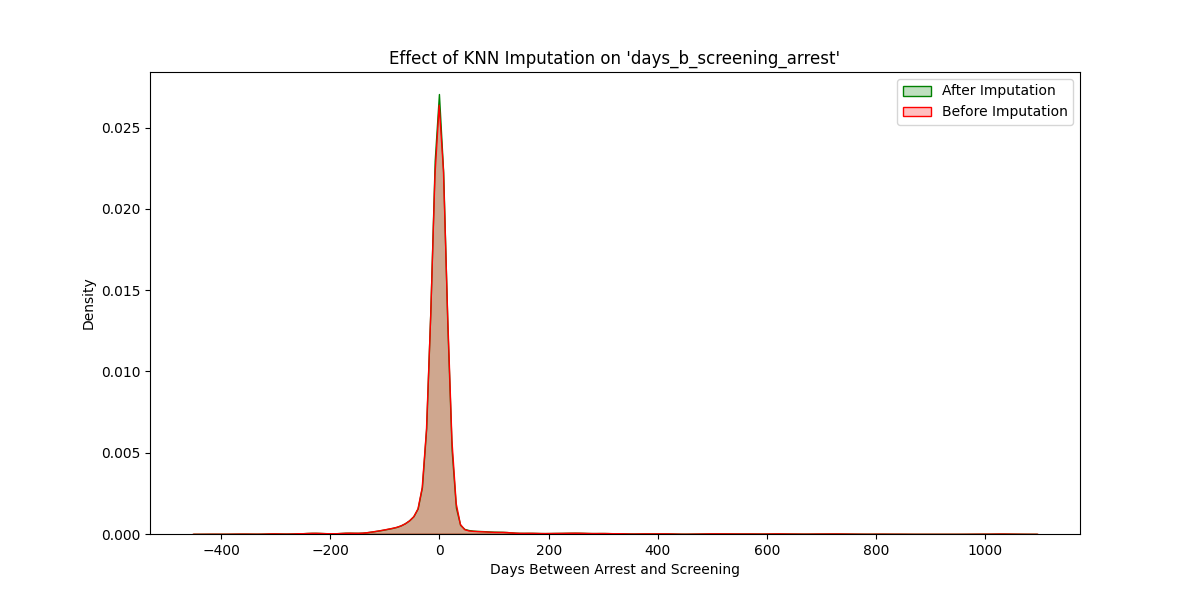
\includegraphics[width=0.9\linewidth]{img/imputation}
	\caption[Distribution \textbf{\texttt{days\_b\_screening\_arrest}} of before and after KNN imputation]{}
	\label{fig:imputation}
\end{figure}

At this stage, the dataset contains four categorical features that need encoding for machine learning algorithms. This section will focus on converting them into a numerical format using two encoding techniques. The categorical features and their values are listed below:

\begin{table}[!ht]
	\centering
	\begin{tabular}{|l|l|l|}
		\hline
		Feature & Description & Unique Values \\ \hline\hline
		\textbf{\texttt{sex}} & Gender of the individual & \shortstack{Male\\Female} \\ \hline
		\textbf{\texttt{race}} & Race of the individual & \shortstack[l]{African-American\\Caucasian\\Hispanic\\Asian\\Native American\\Other} \\ \hline
		\textbf{\texttt{age\_cat}} & Age category & \shortstack[l]{Less than 25\\25 - 45\\Greater than 45} \\ \hline
		\textbf{\texttt{c\_charge\_degree}} & \shortstack{Degree of the\\criminal charge} & \shortstack[l]{F (Felony)\\M (Misdemeanor)} \\ \hline
	\end{tabular}
\end{table}

The following transformations are applied:

\begin{itemize}[]
	\item One-Hot Encoding on \textbf{\texttt{sex}}, \textbf{\texttt{race}}, and \textbf{\texttt{c\_charge\_degree}}, transforming them into binary columns.
	\item Ordinal Encoding on \textbf{\texttt{age\_cat}}. This encoding technique was preferred over one-hot in this case as it preserves order, thus respecting the inherent ranking of the category.
\end{itemize}

The original categorical columns were retained in the dataset for future use in the analysis steps. 

\subsection{Splitting the data into train, test and dev}

A stratified shuffle split technique is preferred to create the train, test, and dev datasets whilst ensuring that the splits are proportional by \textbf{\texttt{race}}. In the first split, 80\% Train and 20\% Test are created, whilst in the Second split, The 20\% Test is further divided into 10\% Test and 10\% Dev.


\section{Data exploration and visualisation}

Here we will examine the dataset in more detail to understand the patterns, distributions, and relationships. In this exercise, we will use more of the visual tools available through several Python libraries to identify potential biases, explore correlations between variables, and uncover insights that may influence the outcomes of predictive models. 

\subsection {Demographic analysis}

We begin this analysis by segmenting the dataset based by race and gender.





\begin{figure}[H]
	\centering
	% First image
	\begin{subfigure}[b]{0.45\linewidth}
		\centering
		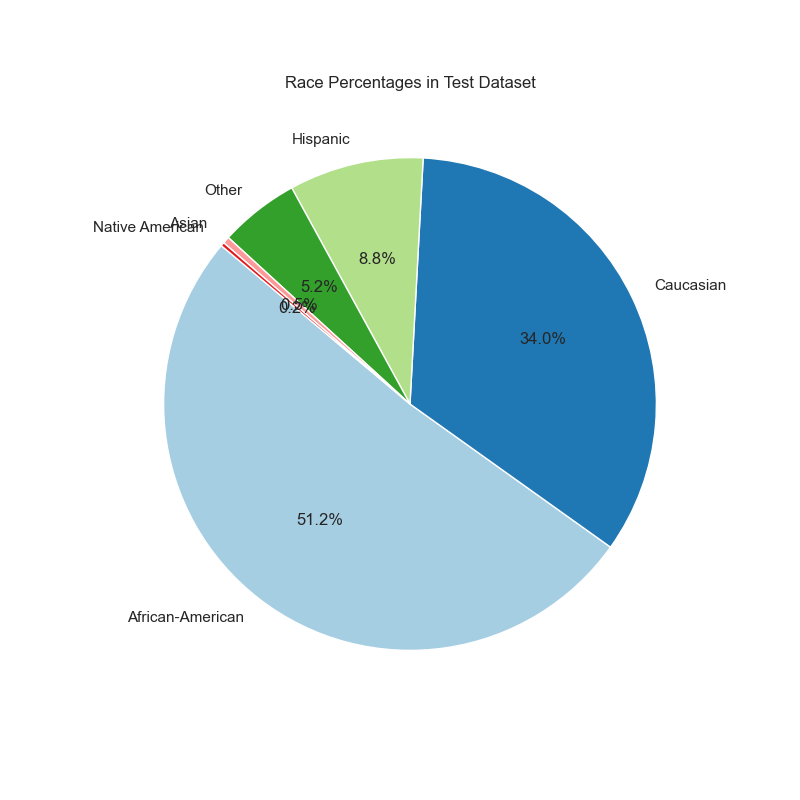
\includegraphics[width=\linewidth]{img/race_percentages_pie.png}
	\end{subfigure}
	\hfill
	% Second image
	\begin{subfigure}[b]{0.45\linewidth}
		\centering
		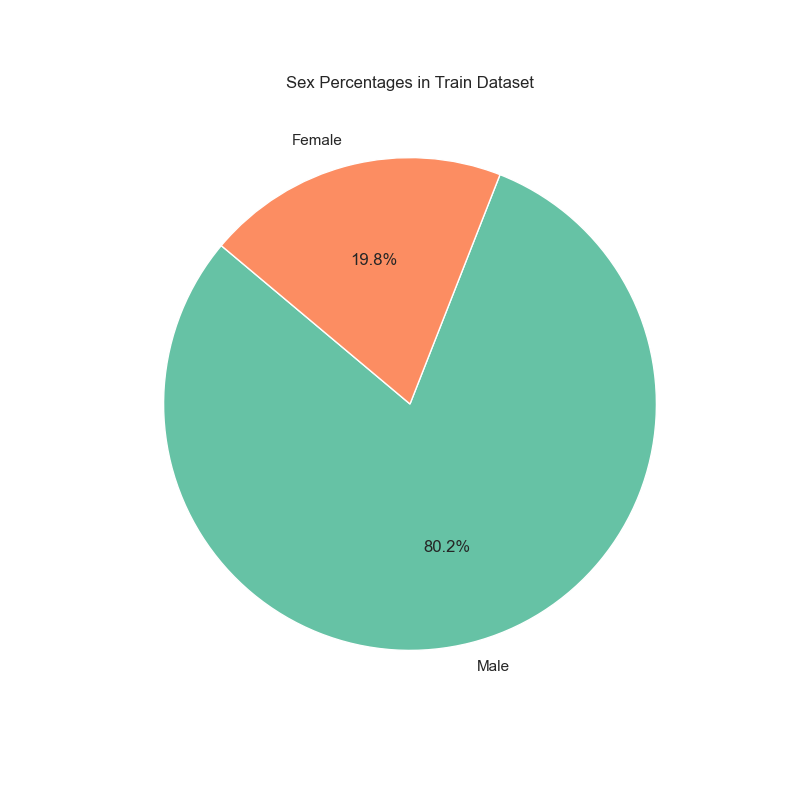
\includegraphics[width=\linewidth]{img/sex_percentages_pie.png}
	\end{subfigure}
	\caption{Race and Sex breakdown for the dataset.}
	\label{fig:race-sex-breakdown}
\end{figure}


%% First image
%\begin{figure}
%	\centering
%	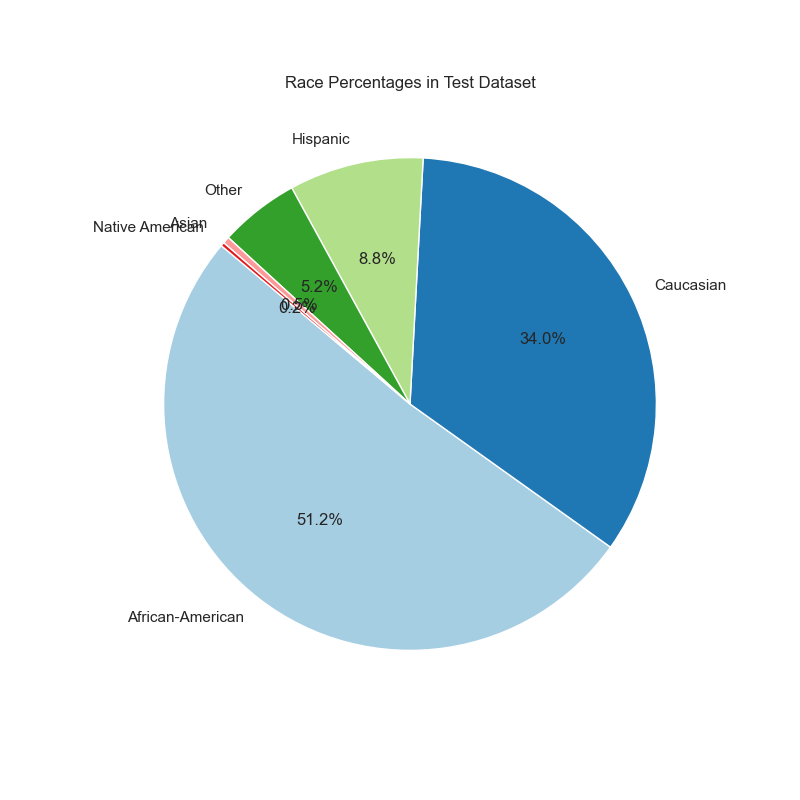
\includegraphics[width=0.7\linewidth]{img/race_percentages_pie.png}
%	\caption{Caption for the first image}
%	\label{fig:image1}
%\end{figure}
%\hfill
%% Second image
%\begin{figure}
%	\centering
%	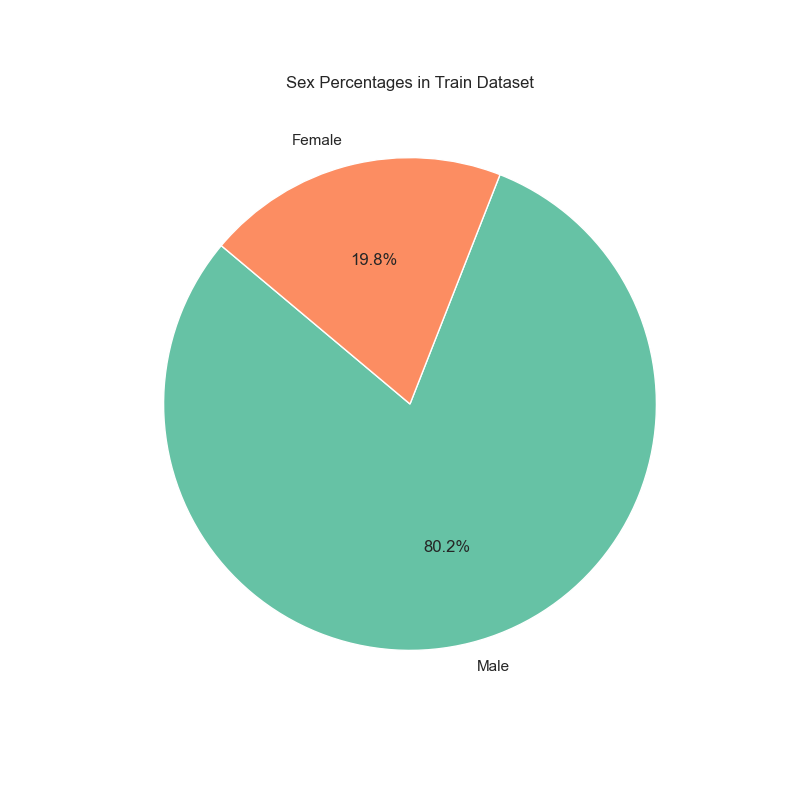
\includegraphics[width=0.7\linewidth]{img/sex_percentages_pie.png}
%	\caption{Caption for the second image}
%	\label{fig:image2}
%\end{figure}


By examining the racial composition of the dataset, we observe the following:

\begin{itemize}
	\item Over half of the test dataset is composed of African-American individuals, suggesting that the dataset may be imbalanced, with a disproportionate representation of one racial group.
	\item Asians and Native Americans each makeup only 0.2\% of the dataset; this underrepresentation might raise some concerns as it may lead to challenges in statistical analysis or machine learning models. Such concerns include the lack of reliability or significance for these groups due to insufficient data.
\end{itemize}

Figure \ref{fig:race-sex-breakdown} also shows our dataset's male/female split, with females comprising only 19.8\%. It is, therefore, evident that the female group is underrepresented, which can lead to biased models as models may overfit male patterns and underperform on females and misleading conclusions as insights derived might generalise poorly for the female subgroup.


\subsection{Age distribution analysis}


We used a boxplot to illustrate the age patterns across racial groups, helping to identify central values, spread, and any anomalies.

\begin{figure}[H]
	\centering
	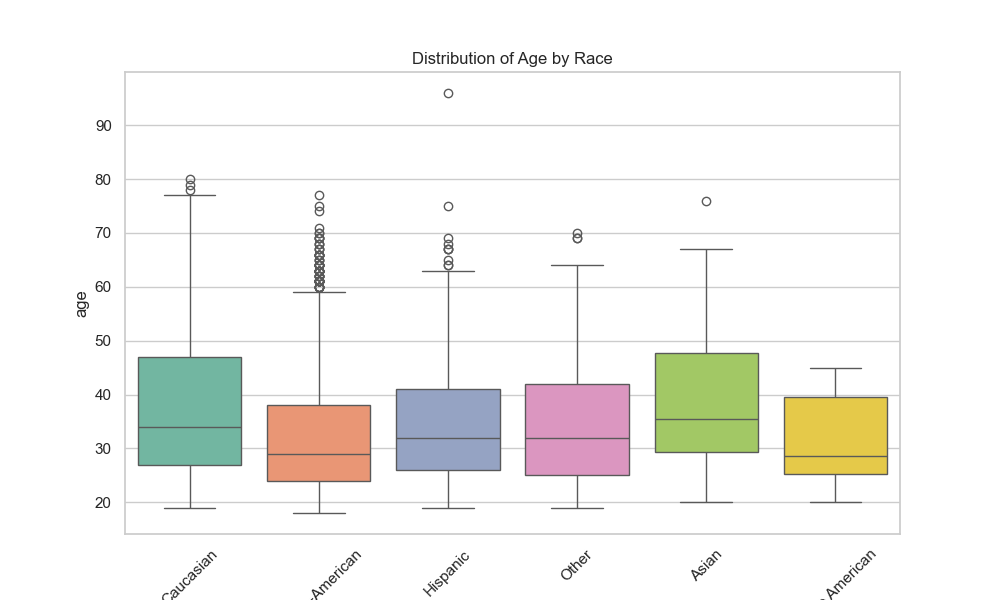
\includegraphics[width=0.9	\linewidth]{img/age_by_race_boxplot}
	\caption{}
	\label{fig:age-by-race-boxplot}
\end{figure}



\begin{table}[H]
	\centering
	\begin{tabular}{|l|l|p{4cm}|}
		\hline
		Race & Median Age & Distribution Description \\ \hline \hline
		African-American & $\approx$30 years & Concentrated in the 20–40 range, with a relatively narrow spread. We notice outliers above 60 years,  indicating fewer older individuals. \\ \hline
		Caucasian & $\approx$40 years & Broader age range, from 20 to 70+ years. We notice more older individuals (upper outliers), making this group appear older on average. \\ \hline
		Hispanic & $\approx$30–35 years & Moderately broad spread, with most individuals between 20 and 50 years. \\ \hline
		Asian & $\approx$30 years & Narrow distribution, concentrated between 25 and 40 years. No outliers. \\ \hline
		Native American & $\approx$33 years & Very tight distribution, with all ages clustered closely around the median (little variability). It is important to note that this group accounts for a tiny portion of the population. \\ \hline
		Other & $\approx$35–40 years & Similar to Caucasians but with slightly fewer older individuals. The IQR shows a widespread. \\ \hline
	\end{tabular}
\end{table}



\subsection{Analysing distributions}


Next, we plotted the distributions of all the features in our dataset; this is depicted in Figure \ref{fig:distribution-plots} . From these histograms, we notice 
\begin{itemize}
	\item The age distribution shows a right-skewed pattern, with most individuals falling in the younger age ranges (20–40 years).
	
	\item There is a significant over-representation of certain racial groups, particularly African Americans, which could indicate potential biases in the dataset's sampling.
	
	\item Most individuals have zero juvenile felony counts, zero juvenile misdemeanour counts, and no recorded "other" juvenile offences, with each distribution rapidly declining for higher counts.
	
	\item A large proportion of individuals have a low number of prior offences, but there is a long tail indicating some individuals have a significant number of priors.
	
	\item Most individuals have relatively short jail durations, with a few experiencing significantly longer durations.
	
	\item The distribution of days between screening and arrest is clustered around zero, with few extreme outliers on both ends.
	
	\item The decile scores appear relatively evenly distributed, but slight patterns suggest clustering at specific score levels (e.g., lower decile scores are slightly more frequent).
	
	\item Two-year recidivism plot shows a near-equal distribution, indicating a balanced dataset for recidivism outcomes.
\end{itemize}


\begin{figure}[H]
	\centering
	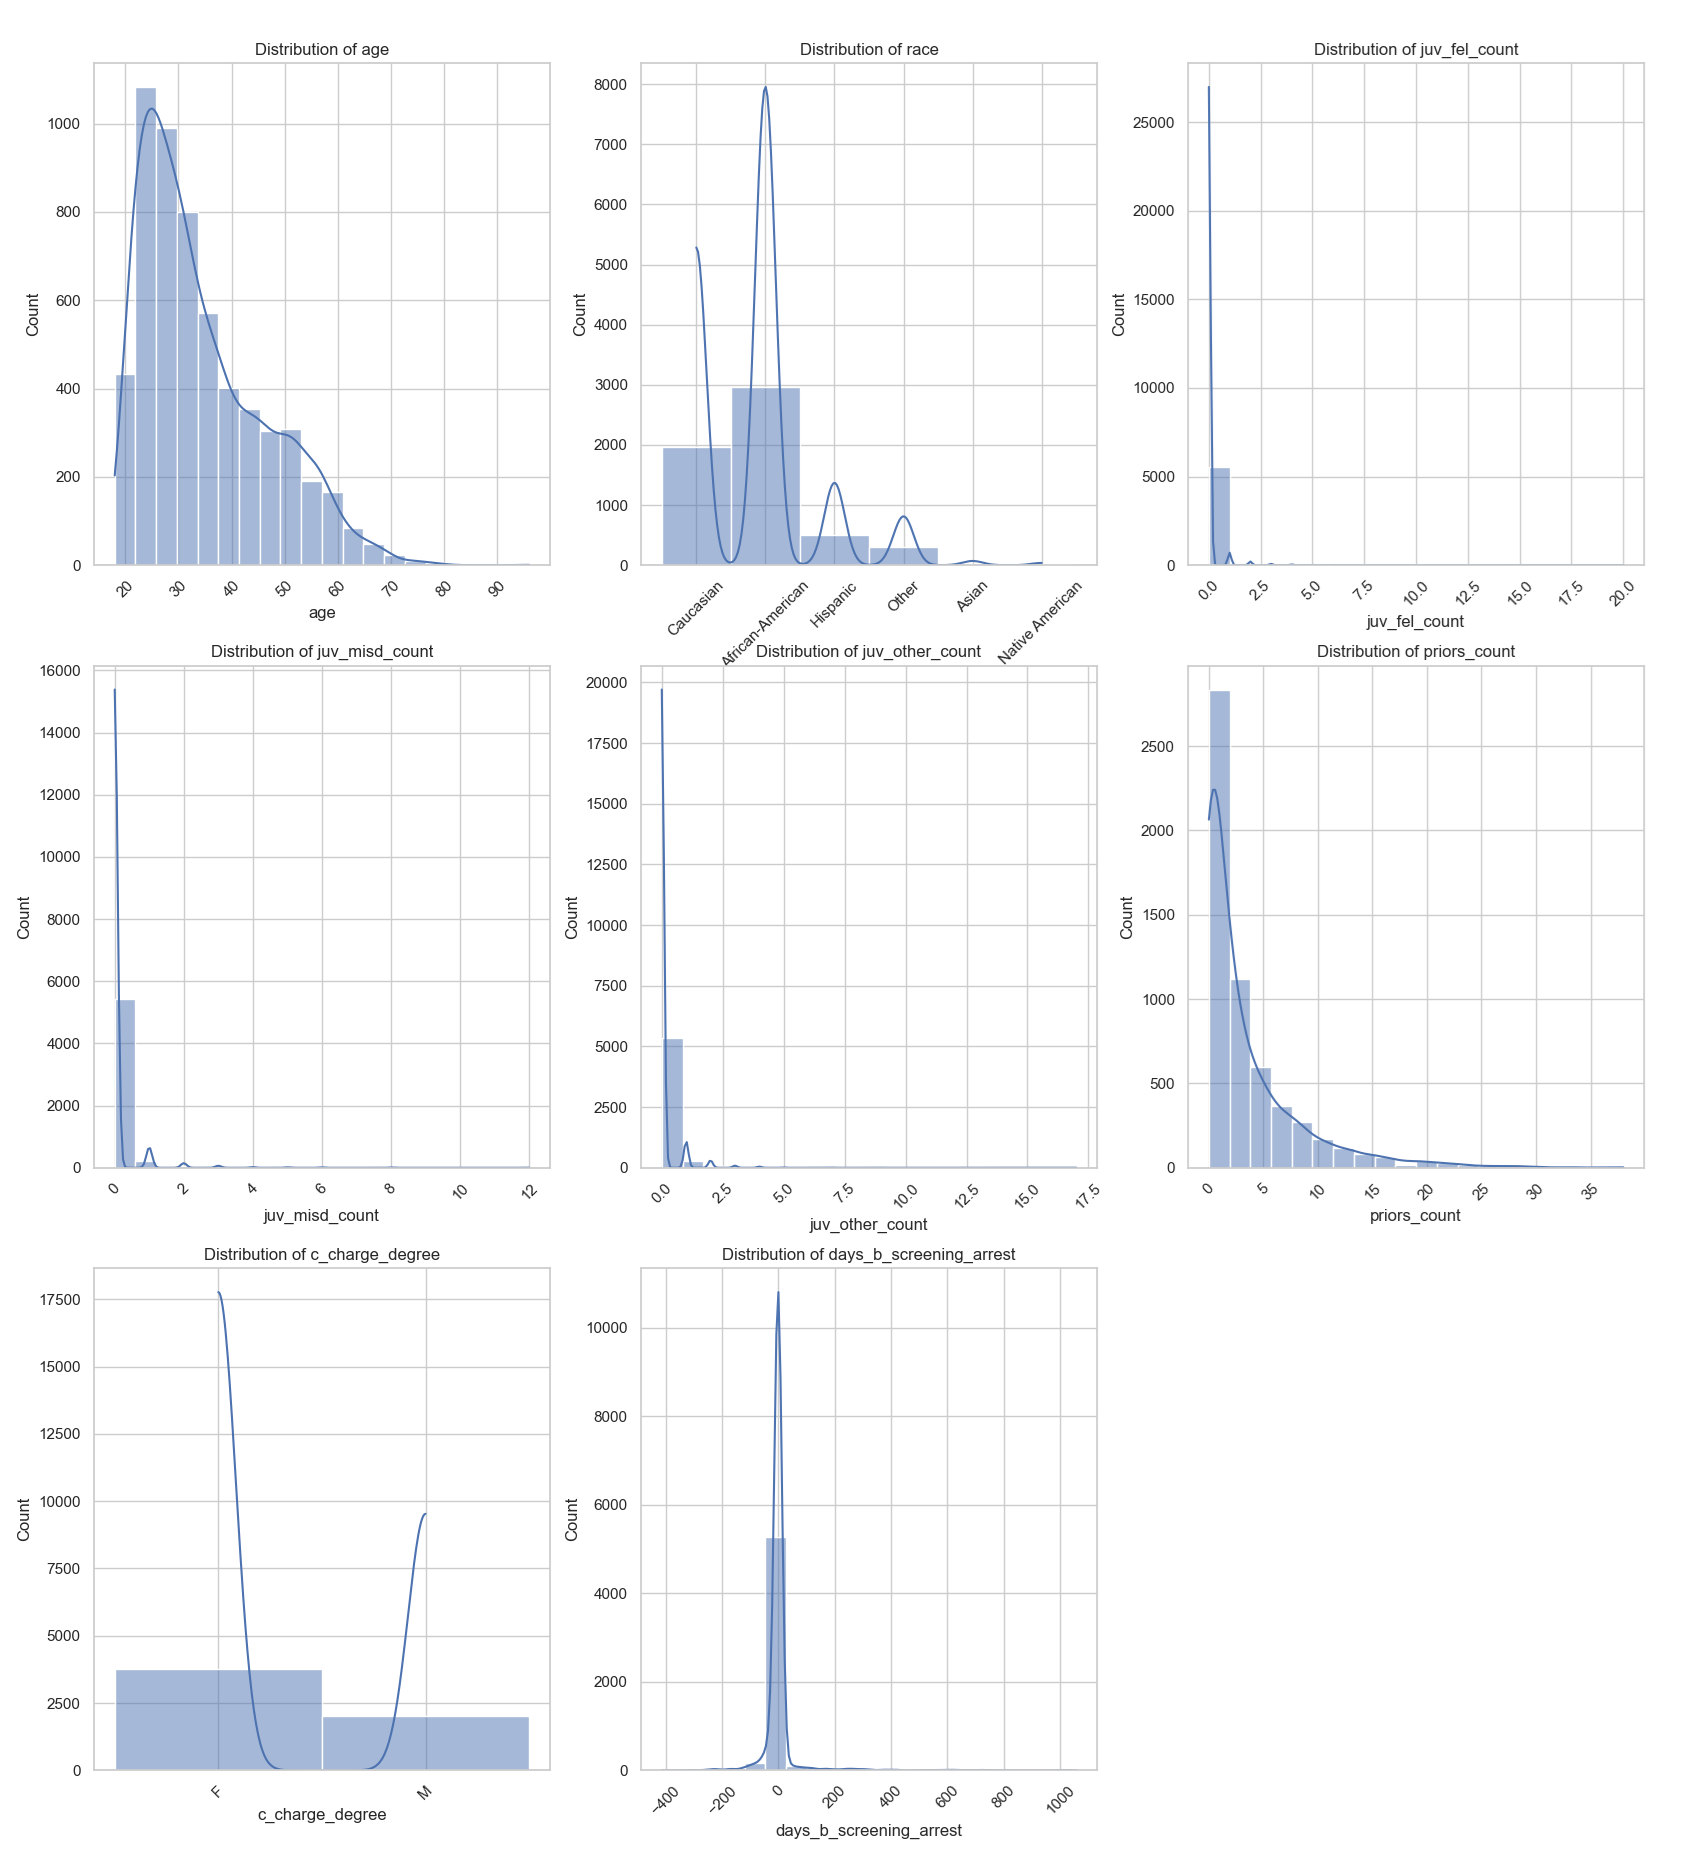
\includegraphics[width=0.9\linewidth]{img/distribution-plots}
	\caption{}
	\label{fig:distribution-plots}
\end{figure}


\subsection{Correlation analysis}

The correlation matrix heatmap shown in Figure \ref{fig:correlationmatrixheatmap} was created to gather more insights and pinpoint the areas of high correlation. This plot raises a number of interesting observations, namely:

\begin{figure}[!h]
	\centering
	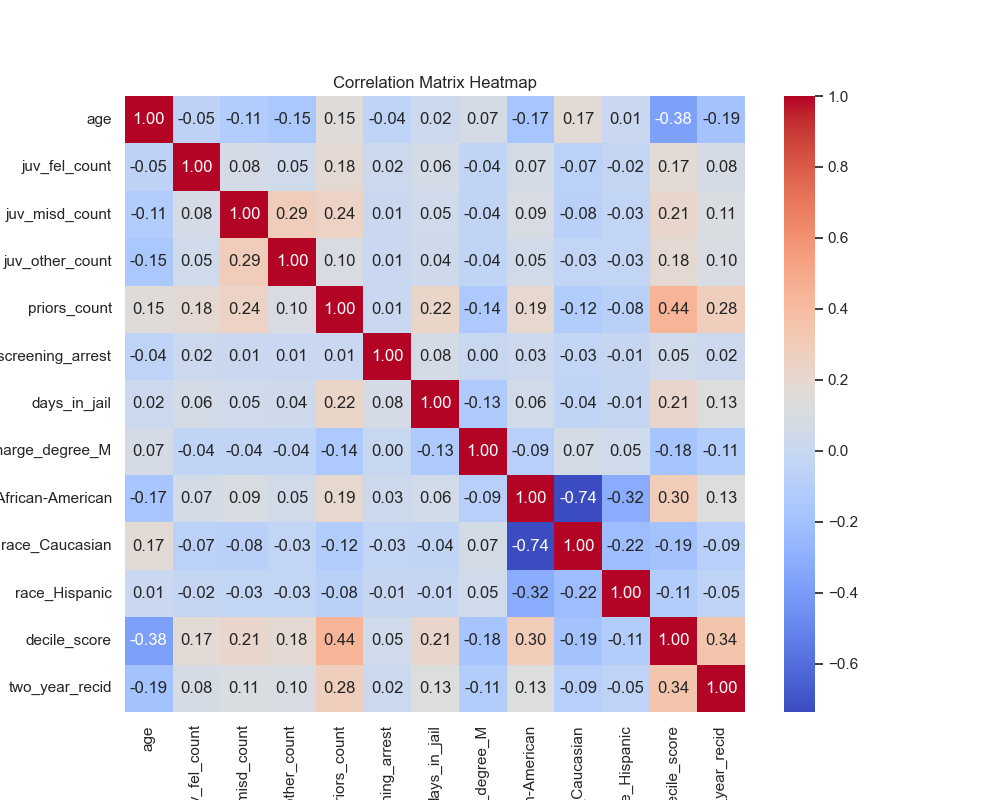
\includegraphics[width=0.7\linewidth]{img/correlation_matrix_heatmap}
	\caption{}
	\label{fig:correlationmatrixheatmap}
\end{figure}


\begin{itemize}
	\item Individuals with more prior offences tend to have higher risk scores, as prior criminal behaviour is a key factor in risk assessment models. The number of prior offences also correlates positively with recidivism; individuals with more prior offences tend to re-offend more often.
	
	\item Older individuals tend to have lower risk scores, suggesting that age may be inversely related to the risk of recidivism, with younger individuals being assessed as higher risk. In addition, older individuals are also less likely to recidivate, supporting this general trend.
	
	\item Individuals with higher risk scores are likelier to recidivate within two years, suggesting that the risk score (\textbf{\texttt{decile\_score}}) is predictive to a certain extent of recidivism.
	
	\item A correlation of 0.30 indicates that being African-American is moderately associated with higher decile scores, raising potential concerns about racial bias in the scoring system. At the same time, Caucasian individuals correlate -0.19 and, therefore, are less likely to receive higher risk scores.
	
	\item The time spent in jail has only a small positive relationship with the likelihood of re-offending within two years
	
	\item  Juvenile felony, misdemeanour, and other counts are positively correlated, indicating that individuals with one type of juvenile record will often have other types.
\end{itemize}

Figure \ref{fig:pairplot} is a pair plot created to substantiate these observations further to show the relationships among the selected numerical features, with the recidivism outcome (\textbf{\texttt{two\_year\_recid}}) as the hue.

\begin{figure}
	\centering
	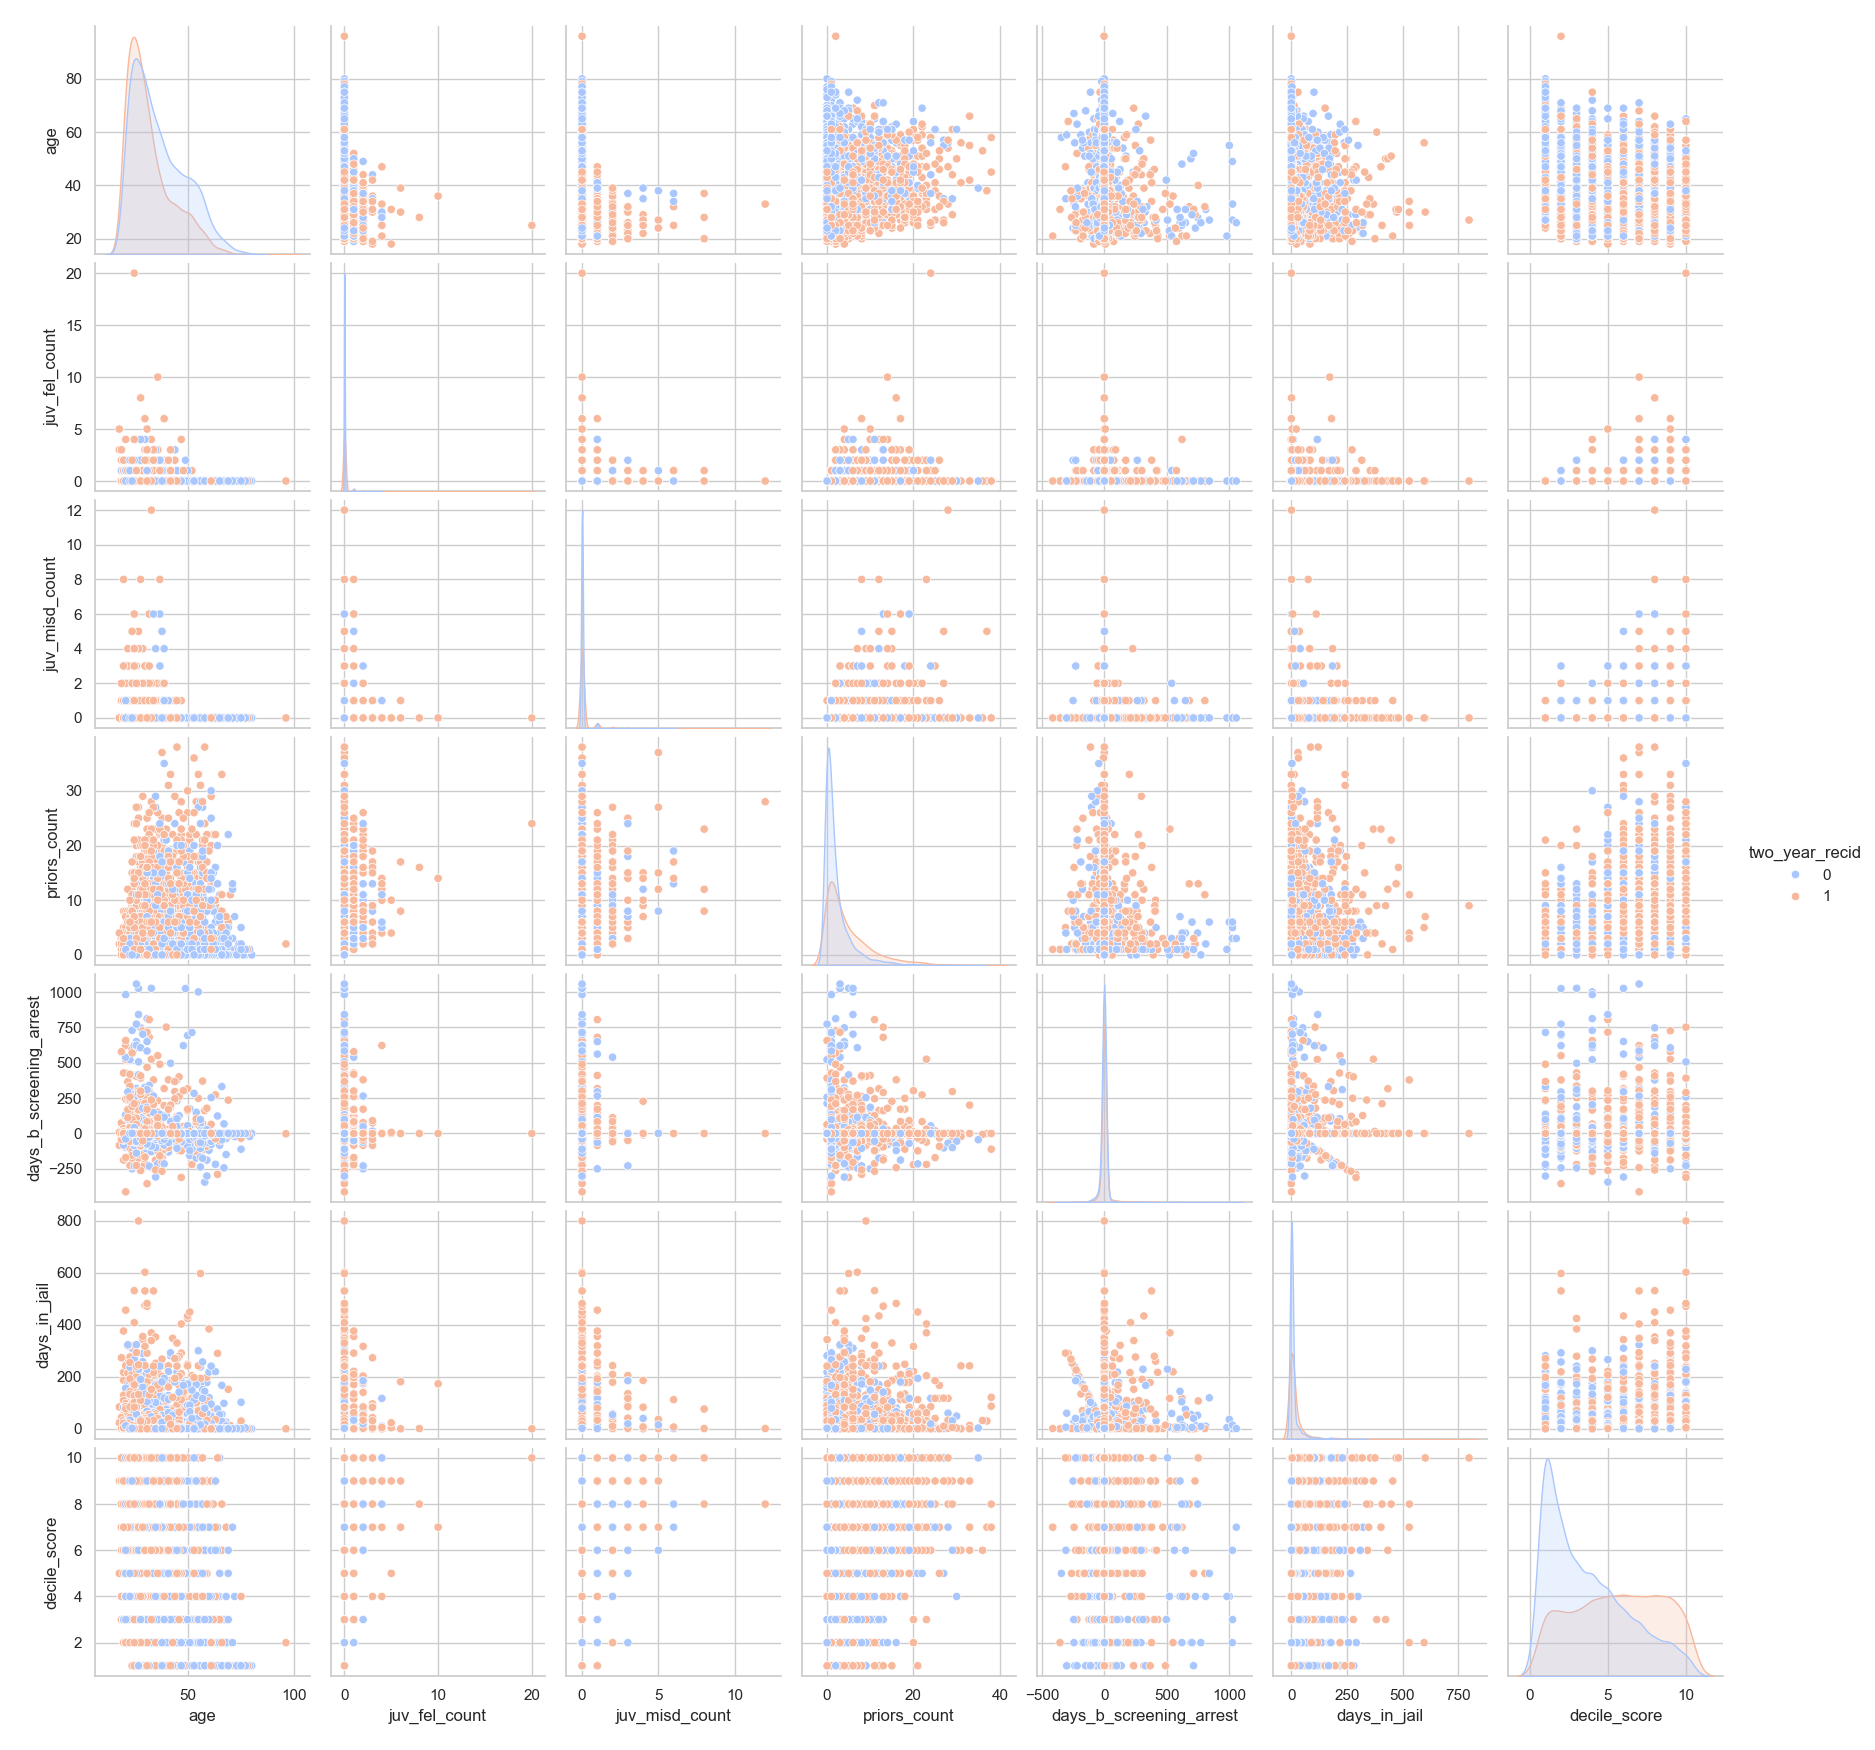
\includegraphics[width=0.7\linewidth]{img/pair_plot}
	\caption{}
	\label{fig:pairplot}
\end{figure}


\begin{itemize}
	\item \textbf{\texttt{age}} vs \textbf{\texttt{priors\_count}}. Younger individuals tend to have fewer prior offences, but the prior count is scattered as age increases, showing that younger offenders tend to continue having problems with the judicial system.
	
	\item \textbf{\texttt{age}} vs \textbf{\texttt{decile\_score}}. Older individuals tend to have lower decile scores. Younger individuals are associated with higher scores.
	
	\item \textbf{\texttt{priors\_count}} vs \textbf{\texttt{decile\_score}}. Positive trend: Higher priors count leads to higher decile scores, suggesting a strong correlation, indicating the tendency for offenders to be viewed as a risk community    
	
	\item The distribution of \textbf{\texttt{decile\_score}}. Two-year recidivists tend to cluster at higher decile scores (6–10 range). Non-recidivists are spread more evenly across scores.        
\end{itemize}



\subsection{Analysis of decile score relationship with race}

The COMPAS dataset has been extensively discussed in recent years regarding the fairness of the scores assigned to individuals, especially considering the race component. Although the tool does not use race as one of the features in decile score prediction, there are concerns that race can be associated indirectly with other features. In this section, we will look at the data from the race point of view to see what patterns we can deduce from the dataset.

As a first step, we create a boxplot to compare the distribution of \textbf{\texttt{decile\_score}} across different racial groups. 

\begin{figure}
	\centering
	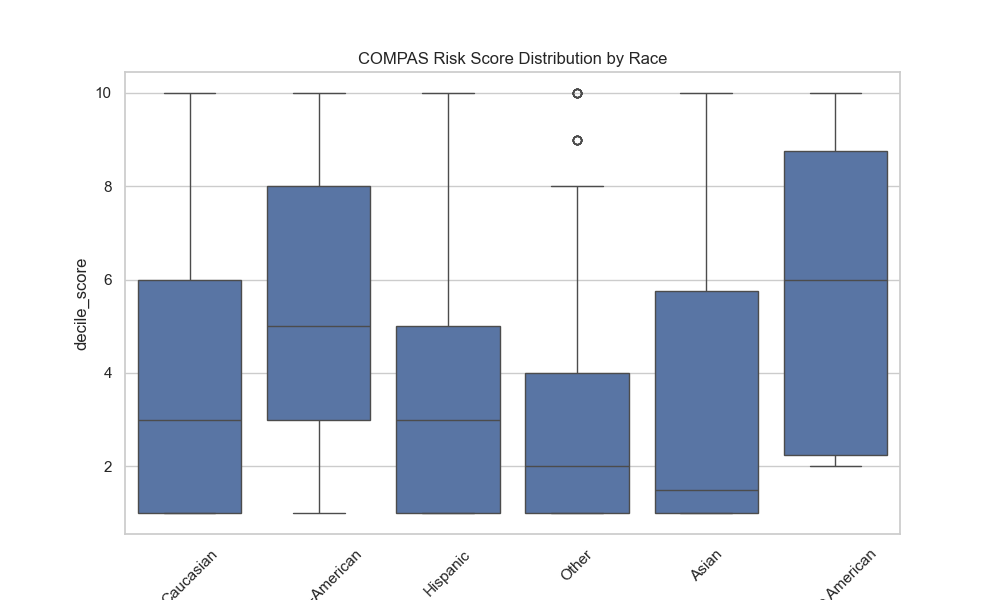
\includegraphics[width=0.7\linewidth]{img/decile_score_by_race_boxplot}
	\caption{}
	\label{fig:decilescorebyraceboxplot}
\end{figure}


From this plot, we notice that African Americans have higher median scores and broader distributions, which suggests a potential bias in the COMPAS scoring system. In addition, Hispanics, Asians, and Other groups scored lower on average, which may indicate differences in the risk assessment process or underlying data inputs.


We then investigated the correlation of \textbf{\texttt{decile\_score}} with \textbf{\texttt{two\_year\_recid}} by race:

\begin{figure}
	\centering
	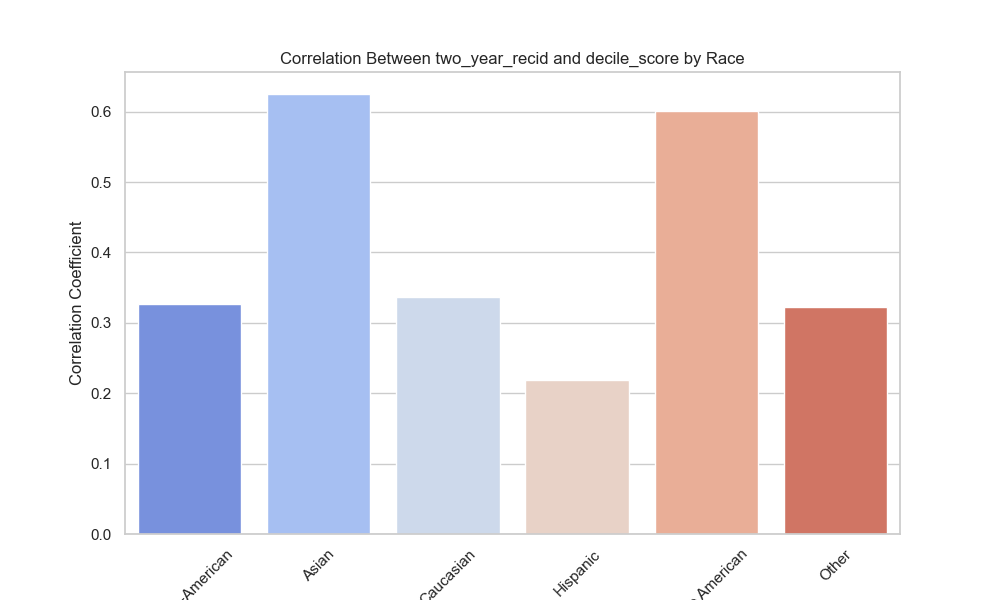
\includegraphics[width=0.9\linewidth]{img/correlation_by_race}
	\caption{}
	\label{fig:correlationbyrace}
\end{figure}

\begin{itemize}
	\item Asians and Native Americans show the highest correlations, indicating that, for these groups, COMPAS scores align more closely with observed recidivism outcomes. However, it is important to remember that these groups comprise a tiny percentage of the population.
	
	\item African-Americans, Caucasians, and Others have moderate correlations, so COMPAS scores are somewhat predictive for these groups but not as strongly as for Asians or Native Americans.
	
	\item The correlation between \textbf{\texttt{two\_year\_recid}} and \textbf{\texttt{decile\_score}} for Hispanics is 0.22, the lowest among the groups, suggesting that for Hispanic individuals, the COMPAS scores are less predictive of actual recidivism outcomes than other racial groups. The low correlation for the Hispanic group is an area of concern because if the COMPAS scores do not accurately predict recidivism for this ethnicity, this could mean that the scoring system may overestimate or underestimate their actual risk, which could lead to misclassification of individuals, leading to potential unfair treatment, for example, harsher parole conditions, sentencing).
\end{itemize}

The distribution of \textbf{\texttt{decile\_score}} for Hispanic individuals was then compared with that of other racial groups using kernel density plots (KDE). 

\begin{figure}
	\centering
	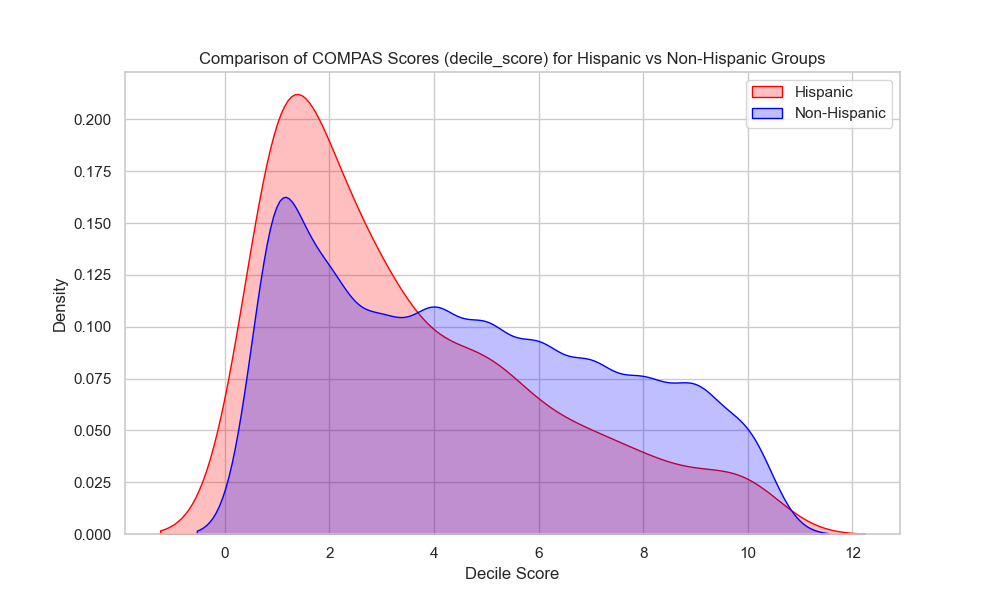
\includegraphics[width=0.7\linewidth]{img/decile_score_by_race_hispanic}
	\caption{}
	\label{fig:decilescorebyracehispanic}
\end{figure}


The plots show that the peak density for Hispanic individuals occurs at a lower score of around 2. In contrast, non-Hispanic individuals have a flatter distribution extending to higher scores, albeit peaking in the same region, suggesting that Hispanic individuals are more likely to receive lower COMPAS scores than non-Hispanic individuals.

One has to note that we have previously seen that Hispanic individuals account for 8.8\% of the population, which is significantly smaller compared to African-American and Caucasian groups.
Although by any means not conclusive, these aspects raise questions about how risk scores are calibrated for underrepresented groups.

\subsubsection{Analysis of the African-American sector}


We created another density plot to compare the distribution of risk scores between African-American individuals and non-African-American individuals.

\begin{figure}
	\centering
	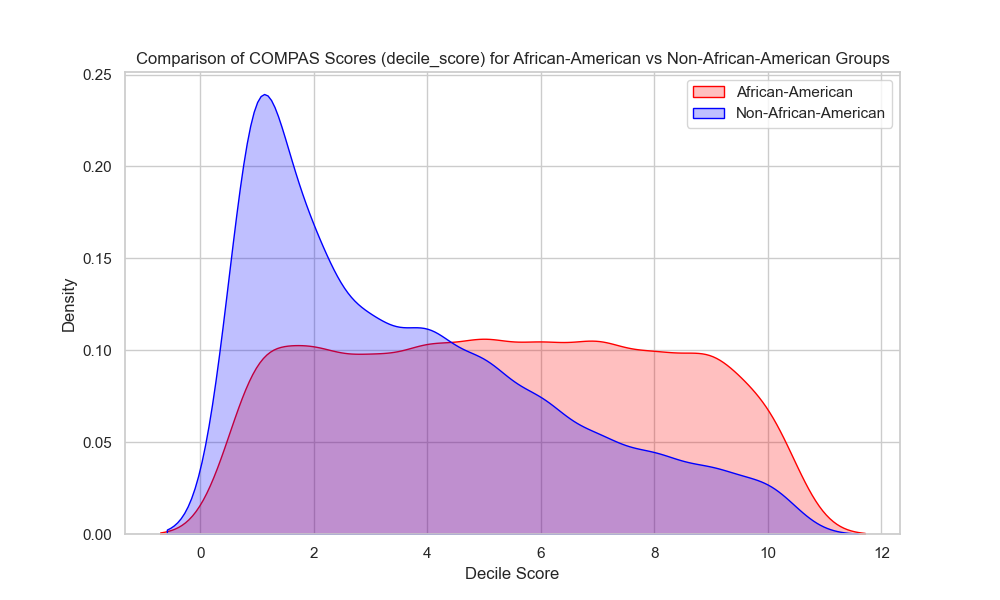
\includegraphics[width=0.7\linewidth]{img/decile_score_by_race_african_american}
	\caption{}
	\label{fig:decilescorebyraceafricanamerican}
\end{figure}


Here, we notice that African Americans are more likely to receive risk scores in the higher decile range, exceeding a value of six, than non-African Americans, suggesting that the COMPAS tool systematically assigns higher risk scores to African Americans. As noticed previously, non-African-American individuals show a strong peak at around a score of 2, with fewer individuals in this group receiving scores in the higher ranges.

This disparity in score distributions raises concerns about potential bias in the COMPAS scoring system. African Americans appear to be disproportionately classified as higher risk, a factor which could impact downstream decisions such as sentencing or parole.

\subsection{Robustness of \textbf{\texttt{decile\_score}}}

As a final analysis, we compare \textbf{\texttt{decile\_score}} with \textbf{\texttt{two\_year\_recid}} to see how many high-risk individuals receded and how many individuals categorised as low-risk did not. This metric is very powerful, as it assesses the validity of the predicted risk metric. Throughout this study, we will also use this test to validate our predicted scores for the machine learning models.


An important decision in this exercise is the selection of the decile score threshold that will dictate that values above it are more likely to recidivate and those below it not. In order to do this, we compared the decile score and two-year record for multiple thresholds. We examined the number of true negatives (the individuals with a decile score lower than the threshold and did not recidivate), true positives (those with a decile score higher or equal than the threshold and did recidivate) and false positives and negatives. We then used these results to calculate the sensitivity, specificity, precision and accuracy:

\begin{table}[h!]
	\centering
	\begin{tabular}{|c|c|c|c|c|}
		\hline
		\textbf{Threshold} & \textbf{Sensitivity} & \textbf{Specificity} & \textbf{Precision} & \textbf{Accuracy} \\ \hline
		4                               & 0.628659             & 0.670551             & 0.60941            & 0.651707          \\ \hline
		5                               & 0.521186             & 0.766299             & 0.645823           & 0.656039          \\ \hline
		6                               & 0.411017             & 0.83811              & 0.674889           & 0.645989          \\ \hline
		7                               & 0.3047               & 0.897323             & 0.708147           & 0.63074           \\ \hline
		8                               & 0.196071             & 0.938268             & 0.721986           & 0.604401          \\ \hline
	\end{tabular}
	\caption{Performance Metrics for Different Decile Score Thresholds}
	\label{tab:performance_metrics}
\end{table}

Following this procedure, a threshold of 5 was decided to provide the best balance of these metrics. With this threshold, the total accuracy and precision are moderate, indicating that while the model performs reasonably well overall, there is room for improvement. We notice a low sensitivity compared to specificity; the model is better at identifying non-recidivists than recidivists.


The metrics for each racial group were then calculated with this threshold.


The Caucasian group has a relatively high specificity but low sensitivity, indicating the COMPAS model more effectively avoids false positives but struggles to identify true positives. 

The African-American group shows higher sensitivity but lower specificity compared to Caucasians. This suggests the model identifies more recidivists among African Americans but at the cost of more false positives.


The Hispanic group has low sensitivity, meaning the model struggles significantly to identify true positives in this group. Precision is also the lowest, indicating a high false-positive rate.


The significant disparity in sensitivity and specificity across racial groups highlights potential fairness issues in the model's predictions. For example, the model disproportionately favours Caucasians and Asians in terms of specificity while penalizing African-Americans with higher false-positive rates.




%pipeline
%--------


\subsection{Preparing data for machine learning}

	Building on the insights derived from the previous section, the next step involved the creation of the pipeline to transform the raw dataset into a format optimized for machine learning models.
	
	\begin{figure}[H]
		\centering
		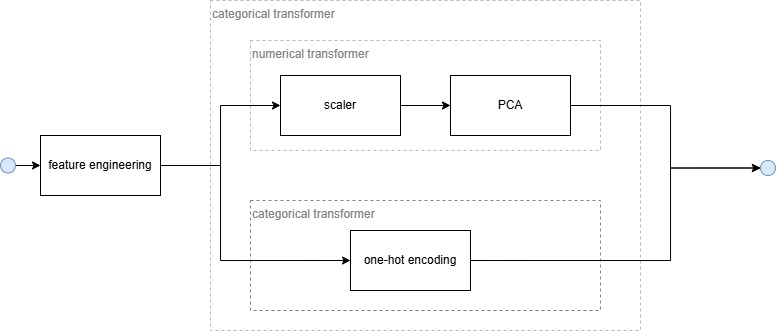
\includegraphics[width=0.7\linewidth]{img/pipeline}
		\caption{}
		\label{fig:pipeline}
	\end{figure}
	
	The pipeline created for this application is shown in Figure \ref{fig:pipeline}. It is based on the \texttt{Pipeline} functionality provided by the Scikit-learn library, integrating feature engineering and transformations for both numerical and categorical data. The pipeline consists of the following components:

	\begin{itemize}
		\item \textbf{Feature Engineering:}
		The pipeline begins with a feature engineering unit where raw features are processed to derive new attributes and filter out irrelevant ones. This step prepares the dataset for subsequent transformations. Feature engineering is based on the Python’s \texttt{pandas} library. The transformation logic was encapsulated in a reusable function, \texttt{feature\_engineering}, which was wrapped in a \texttt{FunctionTransformer} to integrate it into  the machine learning pipeline. 
		
		The primary objective of the feature engineering step is to:
		\begin{itemize}
			\item Retain only the most relevant features for recidivism prediction.
			\item Derive new features to enhance the dataset’s predictive capacity.
			\item Remove unnecessary or redundant columns to reduce noise and complexity.
		\end{itemize}
		
		Following the analysis phase, a subset of the dataset's features was identified as relevant for training and subsequent analysis. These include demographic attributes (e.g., \texttt{age}, \texttt{race}, \texttt{sex}), prior criminal history (\texttt{priors\_count}), juvenile offense counts (\texttt{juv\_fel\_count}, \texttt{juv\_misd\_count}, \texttt{juv\_other\_count}), and timestamps related to jail custody (\texttt{c\_jail\_in}, \texttt{c\_jail\_out}) and general custody (\texttt{in\_custody}, \texttt{out\_custody}). Features such as names and IDs were excluded to avoid introducing irrelevant or sensitive information into the analysis.
		
		We decided to keep the \texttt{race} feature so that we can use it to analyse the results obtained by the machine learning models, but it will be removed from the features set at a later stage.
		
		Two new features were created to capture time-based patterns:
		\begin{itemize}
			\item \textbf{\texttt{days\_in\_jail}}: Calculated as the absolute difference in days between the \texttt{c\_jail\_in} and \texttt{c\_jail\_out} timestamps. This feature provides insight into the duration of incarceration for a given charge.
			\item \textbf{\texttt{days\_in\_custody}}: Calculated as the absolute difference in days between the \texttt{in\_custody} and \texttt{out\_custody} timestamps. This feature reflects the total time an individual spent in custody.
		\end{itemize}
		
		These features offer information about the extent of an individual’s interaction with the criminal justice system, which may correlate with recidivism likelihood. As the originating features  had frequent nulls, zeros were imputed where the calculation did not result into a number.
		
		The final processed dataset contains the following columns:
		\begin{itemize}
			\item \textbf{Demographic Features}: \texttt{sex}, \texttt{age}, \texttt{race}.
			\item \textbf{Juvenile Offense Counts}: \texttt{juv\_fel\_count}, \texttt{juv\_misd\_count}, \texttt{juv\_other\_count}.
			\item \textbf{Criminal History}: \texttt{priors\_count}.
			\item \textbf{Derived Features}: \texttt{days\_in\_jail}, \texttt{days\_in\_custody}.
		\end{itemize}
		
		This feature engineering process resulted in a clean and concise dataset, ready for use in machine learning pipelines. By deriving meaningful features and eliminating irrelevant data, the preprocessing step set a strong foundation for building predictive models.
		
		
		\item \textbf{Numerical transformer:}
		\begin{itemize}
			\item \textbf{Scaler:} Numerical features are standardized or normalized to ensure they are on a similar scale. This step is critical for distance-based algorithms and gradient-based optimization.
			\item \textbf{PCA (Principal Component Analysis):} After scaling, dimensionality reduction is applied to numerical features to eliminate redundancy and reduce the complexity of the data. PCA retains the most important components that explain the majority of variance in the data.
		\end{itemize}
		
		\item \textbf{Categorical Transformer:}
		\begin{itemize}
			\item \textbf{One-Hot Encoding:} Categorical variables are transformed into numerical format using one-hot encoding. This technique creates binary columns for each category, ensuring compatibility with machine learning models.
		\end{itemize}
		
		\item \textbf{Integration of Transformations:}
		The outputs from the \textit{numerical transformer} and \textit{categorical transformer} are combined into a unified dataset using the Scikit-learn pipeline framework. This ensures that the transformations are consistently applied to both training and testing datasets, improving reproducibility and minimizing data leakage.
	\end{itemize}
	
	This pipeline structure allows for the independent processing of numerical and categorical features, enabling specialized transformations for each type of data. The modular design, powered by Scikit-learn’s \texttt{Pipeline} and \texttt{ColumnTransformer}, ensures flexibility and reusability, making it adaptable to various datasets and machine learning workflows. By incorporating scaling, PCA, and encoding, the pipeline ensures the dataset is well-prepared, reducing potential biases or inefficiencies during model training.
	
	This approach represents an effective preprocessing strategy for heterogeneous datasets and highlights the importance of tailored transformations for achieving robust model performance.
	
	\section{Experiments}
	
	We start this investigation by explaining very shortly the project structure for this exercise. Unlike analysis, Python files were used to create the models, tune them and carry out experiments. 
	
	
	\begin{itemize}
		\item A \textbf{utils} area contains all the scripts necessary to download the dataset, split it in train and test datasets, define the feature engineering module and create the preprocessing pipeline. As most of these scripts manipulate the dataset, their result is ultimately saved in a \textbf{data} folder.
		
		\item A \textbf{models} area contains the definition of the k-nearest neighbour, logistic regressor and neural network. In all three model definitions, an initial step is to try and access a 'best parameters' file that contains the result of an optimization step that is described later on in this list. The model is combined with the preprocessor  to create the model pipeline.
		
		\item An \textbf{experiments} area contains all the experiments that are carried out as part of this exercise. It contains three types of modules:
		
		\begin{enumerate}
			\item A script is designed to evaluate the performance of a machine learning pipeline on test data. It computes and reports key metrics, including accuracy, ROC AUC, F1-scores for both classes, precision, overall accuracy, and weighted average F1. The evaluation includes generating and saving a classification report, a confusion matrix visualization, and an ROC curve plot. Results are saved in \textbf{results} folder for further analysis.
			
			\item \textbf{Experiment} scripts for each of the three machine learning methods that is used for training, evaluating, and saving a model pipeline. It loads the training and test datasets, fits the specified model pipeline on the training data, evaluates its performance on the test data using the functions explain previously, and saves the trained pipeline to a file for future use.
			
			\item \textbf{Optimization} scripts that tune our machine learning model pipelines using grid search with cross-validation. After completing the grid search, each script identifies and saves the best parameters and corresponding cross-validation accuracy. It also exports the full results of the grid search as a CSV file for detailed analysis. This process ensures a systematic and reproducible approach to selecting optimal model hyperparameters.
		\end{enumerate}
	\end{itemize}
	
	
	\bigskip
	\subsubsection{Logistic regression experiments}
	
	Logistic regression results demonstrate that the model achieved a test accuracy of approximately 69.5\%, and a ROC AUC of 0.74 as can be seen in Figure \ref{fig:logisticregressionroc}, outperforming the baseline COMPAS results in several key areas. The logistic regression model demonstrated better overall accuracy compared to COMPAS and a higher ROC AUC, indicating improved discriminatory power in separating the two classes. Furthermore, the F1-score for the minority class was significantly higher, reflecting a better balance between precision and recall, particularly for the harder-to-predict positive class.
	
	Examining the confusion matrix show in Figure \ref{fig:logisticregressioncm} further illustrates the logistic regression model's improvements. The tuned model identified fewer false positives and false negatives relative to the COMPAS predictions, suggesting that logistic regression was more effective at minimizing classification errors across both classes. The tuned model demonstrated better precision and recall for class 1, likely due to its capacity for optimization during the tuning phase, whereas COMPAS appears to struggle more with recall, as evidenced by its larger number of false negatives. This is a significant improvement as false negatives correspond to the people that has a high decile score but did not have further encounters with the legal system.
	
	\begin{figure}[H]
		\centering
		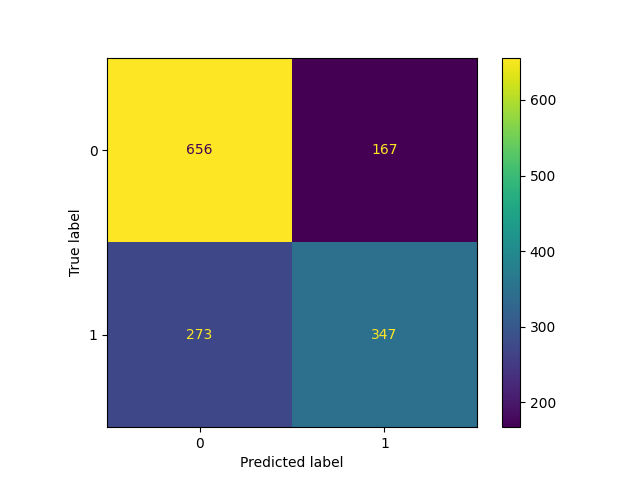
\includegraphics[width=0.7\linewidth]{img/logistic_regression_cm}
		\caption{Confusion matrix for logistic regression model}
		\label{fig:logisticregressioncm}
	\end{figure}
	
	\begin{figure}[H]
		\centering
		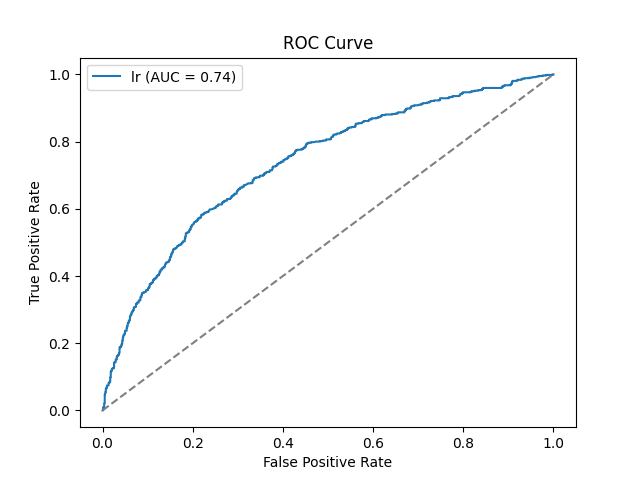
\includegraphics[width=0.7\linewidth]{img/logistic_regression_roc}
		\caption{Receiver operator characteristic plot for logistic regression model}
		\label{fig:logisticregressionroc}
	\end{figure}
	
	
	The \texttt{class\_weight='balanced'} parameter in Scikit-learn's \texttt{LogisticRegression} adjusts the weights of the classes inversely proportional to their frequencies in the training data, effectively addressing class imbalance. By assigning higher importance to the minority class 1, this parameter ensures that the model does not disproportionately favor the majority class 0. As a result, the recall for class 1 improved to 0.67 compared to previous configurations, indicating that the model is better at correctly identifying instances of the minority class. However, this improvement came at a slight cost to precision for both classes, as the model now predicts class 1 more frequently, leading to a lower overall accuracy (67.71\%). 
	
	With the balanced weights, the model's improved recall for the minority class, that individuals who will reoffend,  may lead to better proactive interventions. However, the trade-off is an increase in false positives, which could mean incorrectly labelling individuals as high risk. This could unfairly subject some individuals to harsher penalties
	
	This result highlights the ethical and societal implications of optimizing machine learning models, especially for imbalanced datasets.
	
	
	
	\bigskip
	\subsubsection{K-nearest neighbour experiments}
	
	The k-Nearest Neighbors (kNN) model achieved a test accuracy of 73.46\% and a ROC AUC of 0.80 as can be seen in Figure \ref{fig:knnroc}, which are notable improvements over the COMPAS results and slightly better than the logistic regression model. The precision and recall metrics for class 1 are 0.73 and 0.60, respectively, resulting in an F1-score of 0.66. This performance demonstrates that kNN is more effective at balancing the prediction of both classes, with a better trade-off between precision and recall compared to logistic regression and COMPAS. The ROC AUC score of 0.8 highlights the model’s strong ability to differentiate between the two classes.
	
	Compared to logistic regression, the confusion matrix for kNN, shown in Figure \ref{fig:knncm} shows fewer false positives and a higher number of true positives. This suggests that kNN is better at minimizing classification errors for the majority class while still improving recall for the minority class. Compared to COMPAS, kNN drastically reduces false negatives and false positives, making it a significantly more balanced and fair model for this classification task.
	
	In practical terms, the improved performance of kNN translates to more accurate predictions, particularly for identifying individuals at higher risk. This could lead to better decision-making, reducing the likelihood of unfairly labeling low-risk individuals as high risk while improving the identification of true high-risk cases. 	
	
	
	\begin{figure}[H]
		\centering
		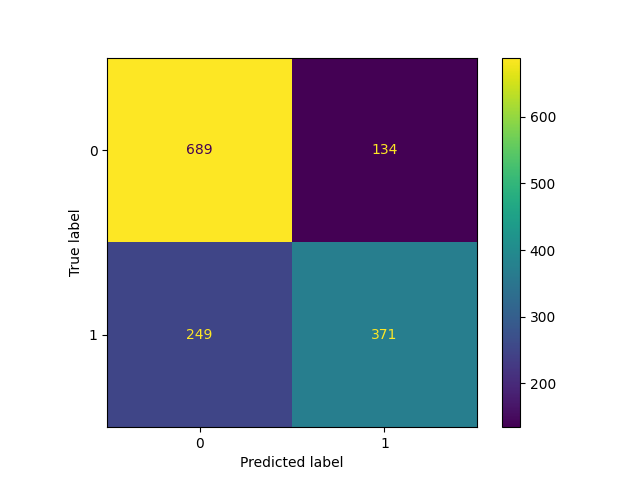
\includegraphics[width=0.7\linewidth]{img/knn_cm}
		\caption{Confusion matrix for k-nearest neighbour model}
		\label{fig:knncm}
	\end{figure}
	
	\begin{figure}[H]
		\centering
		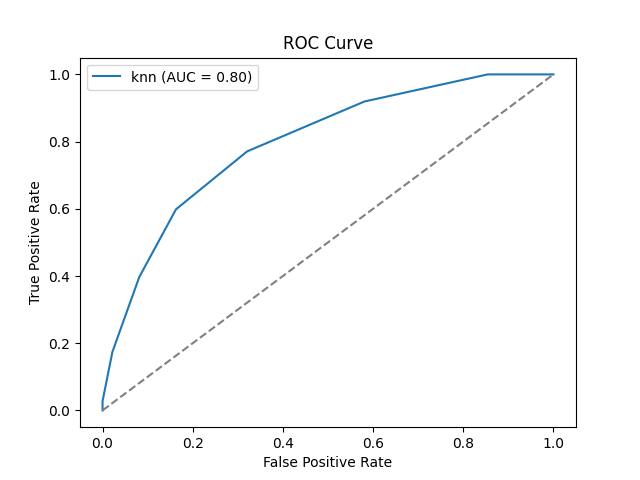
\includegraphics[width=0.7\linewidth]{img/knn_roc}
		\caption{Receiver operator characteristic plot for k-nearest neighbour model}
		\label{fig:knnroc}
	\end{figure}
	
	
	
	The k-Nearest Neighbors (kNN) model configured with \texttt{weights='distance'} demonstrated exceptional performance, achieving a test accuracy of 98\% and a near-perfect ROC AUC score of 0.9991 as can be seen in Figure \ref{fig:knnrocdistance}. By weighting closer neighbors more heavily, the model effectively used local information to make better predictions. According to the classification report, the model achieved a precision of 0.97, recall of 1.00, and F1-score of 0.98 for class 0, and a precision of 1.00, recall of 0.95, and F1-score of 0.98 for class 1. This indicates balanced and superior performance across both classes. As can be seen in Figure \ref{fig:knncmdistance}, the confusion matrix further highlights this improvement, with only 30 misclassified instances.
	
	While these results are remarkable, they also raise important ethical considerations. The dramatic improvement in performance suggests that the model may be overfitting to the training data, particularly since the dataset is relatively small and lacks variability. The use of \texttt{weights='distance'} could amplify biases present in the dataset, as the model prioritizes local data points, which may inadvertently reflect systemic or historical inequalities. In applications such as recidivism prediction, this could lead to overly confident predictions that disproportionately impact certain groups, raising concerns about fairness and accountability. Thus, while the improved performance is promising, careful validation on diverse and representative datasets is necessary to ensure the model's robustness and equitable application.
	
	\begin{figure}[H]
		\centering
		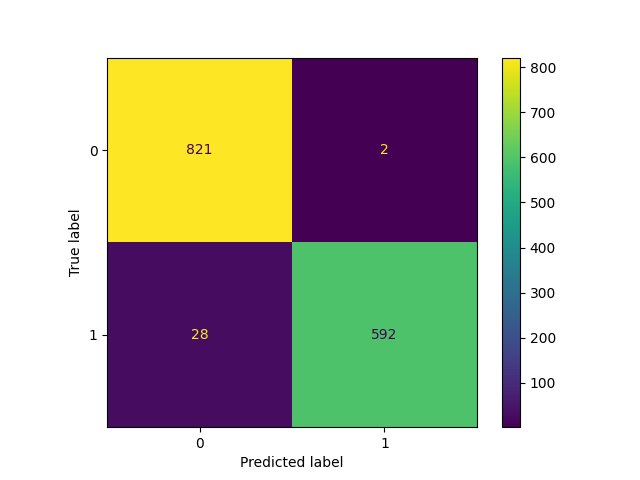
\includegraphics[width=0.7\linewidth]{img/knn_cm_distance}
		\caption{Confusion matrix for k-nearest neighbour model with weights parameter set to distance. This is probably the result of overfitting.}
		\label{fig:knncmdistance}
	\end{figure}
	
	\begin{figure}[H]
		\centering
		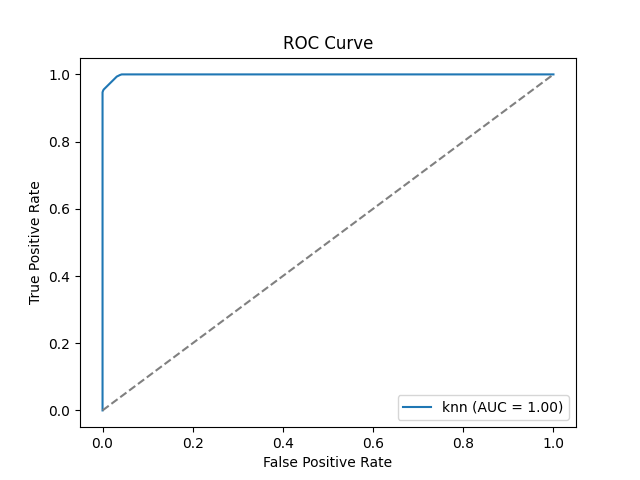
\includegraphics[width=0.7\linewidth]{img/knn_roc_distance}
		\caption{Receiver operator characteristic plot for k-nearest neighbour model with weights parameter set to distance. This is probably the result of overfitting.}
		\label{fig:knnrocdistance}
	\end{figure}
	
	
	\bigskip
	\subsubsection{Neural network experiments}
	
	The neural network implemented in exercise consists of an input layer, followed by two fully connected hidden layers. The first hidden layer contains 128 neurons, and the second contains 64 neurons, each followed by batch normalization and a ReLU activation function. The output layer consists of 2 neurons with a softmax activation function. The model is trained using the cross-entropy loss function, optimized with the Adam optimizer, and employs a mini-batch training strategy with a default batch size of 32 and 20 epochs.
	
	
	The neural network achieved a test accuracy of 70\% and a ROC AUC score of 0.75, reflecting moderate performance in distinguishing between the two classes. The model attained a precision of 0.75, recall of 0.71, and F1-score of 0.73 for class 0, while for class 1, the precision was 0.64, recall was 0.69, and F1-score was 0.66. These metrics highlight that the model performs slightly better for the majority class but still maintains a balanced recall across both classes, which is important in scenarios like this with potential imbalance. The confusion matrix shows 242 false positives and 191 false negatives, indicating that while the model correctly predicts most instances, there is room for improvement.
	
	
		\begin{figure}[H]
		\centering
		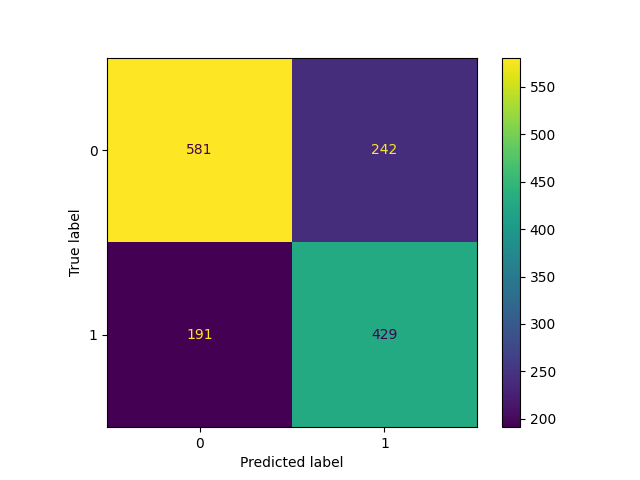
\includegraphics[width=0.7\linewidth]{img/nn_cm}
		\caption{Confusion matrix for neural network model.}
		\label{fig:nncm}
	\end{figure}
	
	\begin{figure}[H]
		\centering
		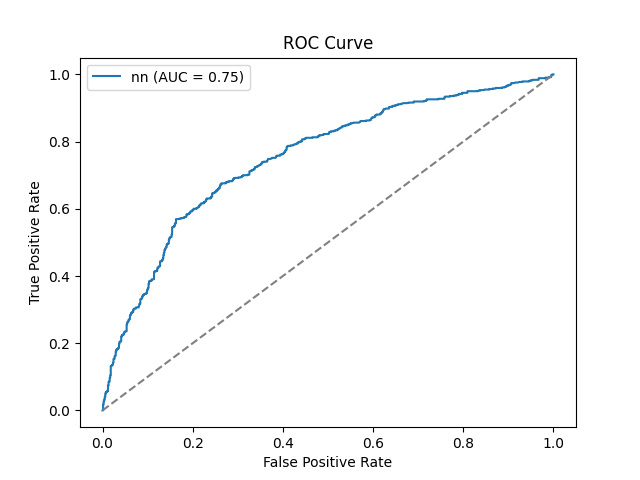
\includegraphics[width=0.7\linewidth]{img/nn_roc}
		\caption{Receiver operator characteristic plot for neural network model.}
		\label{fig:nnroc}
	\end{figure}
	
	
	Changing the loss function to mean squared error caused some differences in how the network performs. While the overall accuracy stayed the same, the model became better at identifying instances of the minority class but less precise when predicting the majority class. This happened because MSE treats errors more evenly, which helps the model focus on reducing overall mistakes rather than just making the most confident predictions.
	
	By using MSE, the model seems to make fairer predictions across both classes, improving recall for the minority class. However, this comes with a trade-off: the model may not be as confident in its predictions. Choosing MSE or another loss function depends on what matters most for the task—whether it's catching as many minority cases as possible or making highly confident predictions.
	
	\subsubsection{Final comments on experiments}
	

	
	Table \ref{tab:metrics} summarizes the performance metrics across the different techniques. Logistic regression (\texttt{lr}) and its class-weighted variant (\texttt{lr balanced}) provide baseline results, with the balanced variant slightly improving recall for the minority class but at the cost of precision and overall accuracy. The weighted F1-score also slightly decreased, reflecting the trade-off in class predictions.
	
		
	\begin{table}[H]
		\centering
		\begin{tabular}{|l|c|c|c|c|}
			\hline
			\textbf{Technique} & 
			\makecell{F1-Score \\Class 0\\Class 1} & 
			\makecell{Precision \\ (Class 1)} & 
			\makecell{Overall\\Accuracy} & 
			\makecell{Weighted\\Avg\\F1-Score} \\ \hline
			lr & \makecell { 0.75 \\ 0.61 } & 0.68 & 0.70 & 0.68 \\ \hline
			lr balanced & \makecell { 0.71 \\ 0.64 } & 0.61 & 0.68 & 0.67 \\ \hline
			knn & \makecell { 0.78 \\ 0.66 } & 0.73 & 0.73 & 0.72 \\ \hline
			knn distance & \makecell { 0.98 \\ 0.98 } & 1.00 & 0.98 & 0.98 \\ \hline
			nn & \makecell { 0.76 \\ 0.62 } & 0.66 & 0.70 & 0.69 \\ \hline
			nn mse& \makecell { 0.72 \\ 0.68 } & 0.63 & 0.70 & 0.70 \\ \hline
		\end{tabular}
		\caption{Performance Metrics for Classification Techniques}
		\label{tab:metrics}
	\end{table}
	
	
	
	The k-Nearest Neighbors (\texttt{knn}) model performed better than logistic regression in both overall accuracy and weighted F1-score, with a significant improvement in capturing minority class instances. The use of distance-based weights (\texttt{knn distance}) led to exceptional performance, with near-perfect metrics across all evaluation categories. However, this result might indicate potential overfitting and should be carefully validated on unseen data before drawing conclusions.
	
	The neural network (\texttt{nn}) achieved comparable performance to logistic regression, with a slight improvement in recall for the minority class. Changing the loss function to mean squared error (\texttt{nn mse}) resulted in a better balance between precision and recall for both classes, leading to a slight improvement in the weighted F1-score compared to the cross-entropy loss variant. This suggests that MSE as a loss function can encourage fairer predictions across classes in certain scenarios.
	
	Overall, \texttt{knn} outperformed \texttt{lr} and \texttt{nn} models in most metrics, with \texttt{nn mse} demonstrating improved balance compared to \texttt{nn}. However, the extremely high metrics of \texttt{knn distance} should be interpreted with caution, as they may not generalize well to unseen data. The choice of model and loss function should depend on the specific application and the importance of precision, recall, and generalization.
	
	
	\subsection{Ethical Review}
		
	The analysis of the data, model performance, and insights generated raises several ethical concerns and societal implications that warrant careful evaluation. First, the dataset used for training likely reflects inherent biases from historical or systemic inequalities, particularly in domains such as recidivism prediction. If the dataset is biased, models trained on it, regardless of their performance metrics, may inadvertently perpetuate or amplify these biases. For instance, minority groups may face disproportionately higher false positive or false negative rates, which could lead to unjust outcomes such as harsher treatment or denied opportunities.
	
	The insights generated by these models also need to be critically examined. While models like \texttt{knn distance} demonstrated near-perfect performance on the test set, such high metrics often indicate overfitting, meaning the model may not generalize well to new or unseen data. Overfitting, combined with biased data, could result in overly confident predictions that fail to account for the complexities of real-world cases. This raises questions about the trustworthiness of these insights, especially in high-stakes decisions that affect individuals' lives.
	
	From a societal perspective, the implications of deploying these models are profound. A model with high false positive rates for the minority class (e.g., labeling individuals as high risk when they are not) can lead to unfair treatment, reinforcing discrimination and systemic inequities. Conversely, high false negative rates (e.g., failing to identify high-risk individuals) could pose public safety concerns. These outcomes highlight the importance of balancing precision and recall while ensuring fairness and transparency in predictions.
	
	To mitigate these ethical risks, several measures are necessary. Regular bias audits should be conducted on the dataset and model outputs to identify and address disparities. Additionally, stakeholders must be involved in the development process to ensure that the models align with societal values and legal standards. Explainability techniques should also be employed to make model predictions more interpretable, allowing decision-makers to understand the rationale behind predictions. Finally, models should be rigorously tested on diverse and representative datasets to ensure robustness and fairness across different demographic groups.
	
	In summary, while the results demonstrate strong technical performance, the ethical considerations of bias, fairness, and societal impact must remain at the forefront. Developing and deploying machine learning models in sensitive domains requires a careful balance between accuracy and equity, with continuous efforts to ensure accountability and mitigate harm.
	
	
	
	


	


	
	
	
	
	
	
	
	

	
	




	
	
	
	
	
	
	
	
	
	
	
	
	
	
	
	
	
	
	
	
	
	
	
	
	
	
	
	
	
	
	
	
	
	
	

	
	

	


	
	
\printbibliography

\onecolumn
\pagebreak
\appendix 
\section{COMPAS dataset fields}

	\begin{table}[!ht]
	\centering
	\begin{tabular}{|l|l|l|l|l|}
		\hline
		Field Name	&	Description	&	Type	&	Options (if Categorical)	&	Used \\ \hline\hline
		\textbf{\texttt{id}}	&	Unique identifier for each individual.	&	Numeric	&	N/A	&	No \\ \hline
		\textbf{\texttt{name}}	&	Full name of the defendant	&	Text	&	N/A	&	No \\ \hline
		\textbf{\texttt{first}}	&	First name of the defendant (anonymized).	&	Text	&	N/A	&	No \\ \hline
		\textbf{\texttt{last}}	&	Last name of the defendant (anonymized).	&	Text	&	N/A	&	No \\ \hline
		\textbf{\texttt{compas\_screening\_date}}	&	Date of the COMPAS assessment.	&	Date	&	N/A	&	Yes \\ \hline
		\textbf{\texttt{sex}}	&	Gender of the defendant.	&	Categorical	&	Male, Female	&	Yes \\ \hline
		\textbf{\texttt{dob}}	&	Date of birth of the defendant.	&	Date	&	N/A	&	No \\ \hline
		\textbf{\texttt{age}}	&	Age of the defendant at the time of assessment.	&	Numeric	&	N/A	&	Yes \\ \hline
		\textbf{\texttt{age\_cat}}	&	Age category of the defendant.	&	Categorical	&	\makecell[l]{Less than 25\\25 - 45\\Greater than 45}	&	Yes \\ \hline
		\textbf{\texttt{race}}	&	Race of the defendant.	&	Categorical	&	\makecell[l]{African-American\\Caucasian\\Hispanic\\Asian\\Native American\\Other}	&	Yes \\ \hline
		\textbf{\texttt{juv\_fel\_count}}	&	Number of juvenile felony offenses.	&	Numeric	&	N/A	&	Yes \\ \hline
		\textbf{\texttt{juv\_misd\_count}}	&	Number of juvenile misdemeanor offenses.	&	Numeric	&	N/A	&	Yes \\ \hline
		\textbf{\texttt{juv\_other\_count}}	&	Number of other juvenile offenses.	&	Numeric	&	N/A	&	Yes \\ \hline
		\textbf{\texttt{priors\_count}}	&	Number of prior offenses (adult and juvenile).	&	Numeric	&	N/A	&	Yes \\ \hline
		\textbf{\texttt{days\_b\_screening\_arrest}}	&	Days between arrest and COMPAS screening.	&	Numeric	&	N/A	&	Yes \\ \hline
		\textbf{\texttt{c\_jail\_in}}	&	Jail booking date for the charge.	&	Date	&	N/A	&	No \\ \hline
		\textbf{\texttt{c\_jail\_out}}	&	Jail release date for the charge.	&	Date	&	N/A	&	No \\ \hline
		\textbf{\texttt{c\_case\_number}}	&	Case number associated with the charge.	&	Text	&	N/A	&	No \\ \hline
		\textbf{\texttt{c\_offense\_date}}	&	Date of the alleged offense.	&	Date	&	N/A	&	No \\ \hline
		\textbf{\texttt{c\_arrest\_date}}	&	Arrest date for the charge.	&	Date	&	N/A	&	No \\ \hline
		\textbf{\texttt{c\_charge\_degree}}	&	Degree of the charge.	&	Categorical	&	\makecell[l]{F (Felony)\\M (Misdemeanor)}	&	Yes \\ \hline
		\textbf{\texttt{c\_charge\_desc}}	&	Description of the charge.	&	Text	&	Free text	&	No \\ \hline
		\textbf{\texttt{is\_recid}}	&	reoffended after COMPAS screening.	&	Binary	&	0 (No), 1 (Yes)	&	No \\ \hline
		\textbf{\texttt{r\_case\_number}}	&	Case number for the re-offense.	&	Text	&	N/A	&	No \\ \hline
		\textbf{\texttt{r\_charge\_degree}}	&	Degree of the re-offense charge.	&	Categorical	&	\makecell[l]{F (Felony)\\M (Misdemeanor)}	&	No \\ \hline
		\textbf{\texttt{r\_charge\_desc}}	&	Description of the re-offense charge.	&	Text	&	Free text	&	No \\ \hline
		\textbf{\texttt{r\_jail\_in}}	&	Jail booking date for the re-offense.	&	Date	&	N/A	&	No \\ \hline
		\textbf{\texttt{r\_jail\_out}}	&	Jail release date for the re-offense.	&	Date	&	N/A	&	No \\ \hline
		\textbf{\texttt{two\_year\_recid}}	&	Label: offense within two years.	&	Binary	&	0 (No), 1 (Yes)	&	Yes \\ \hline
		\textbf{\texttt{decile\_score}}	&	COMPAS risk score (1-10).	&	Numeric	&	1–10	&	Yes \\ \hline
		\textbf{\texttt{score\_text}}	&	Risk category for general recidivism.	&	Categorical	&	Low, Medium, High	&	Yes \\ \hline
		\textbf{\texttt{v\_type\_of\_assessment}}	&	Type of COMPAS assessment conducted.	&	Text	&	Risk of Recidivism	&	No \\ \hline
		\textbf{\texttt{v\_decile\_score}}	&	Violent recidivism COMPAS score (1-10).	&	Numeric	&	1–10	&	No \\ \hline
		\textbf{\texttt{v\_score\_text}}	&	Risk category for violent recidivism.	&	Categorical	&	Low, Medium, High	&	No \\ \hline
		\textbf{\texttt{start}}	&	Start date of the two-year recidivism period.	&	Date	&	N/A	&	No \\ \hline
		\textbf{\texttt{end}}	&	End date of the two-year recidivism period.	&	Date	&	N/A	&	No \\ \hline
		\textbf{\texttt{event}}	&	offense during the two-year period.	&	Binary	&	0 (No), 1 (Yes)	&	No \\ \hline
	\end{tabular}
\end{table}






\end{document}
